\documentclass[9pt]{beamer}
\usetheme{Madrid}
\usecolortheme{default}
\useoutertheme{split}
\useinnertheme{circles}
\setbeamertemplate{headline}{}
\setbeamertemplate{navigation symbols}{}
\setbeamertemplate{footline}[frame number]

\usepackage{lmodern}
\usepackage[utf8]{inputenc}
\usepackage[T1]{fontenc}
\usepackage{amsmath,amssymb,amsfonts,mathrsfs,mathtools,bm}
\usepackage{booktabs}
\usepackage{array}
\usepackage{xcolor}
\usepackage{hyperref}
\usepackage{graphicx}
\usepackage{stmaryrd}

% -----------------------------------------------------------------------------
% Macros
% -----------------------------------------------------------------------------
\def\Xc{{\cal X}}
\def\Ac{{\cal A}}
\def\Tc{{\cal T}}
\def\Pc{{\cal P}}
\def\Lc{{\cal L}}
\def\Rc{{\cal R}}
\def\Sc{{\cal S}}
\def\Gc{{\cal G}}
\def\Jc{{\cal J}}
\def\Nc{{\cal N}}
\def\Uc{{\cal U}}
\def\E{{\mathbb E}}
\def\P{{\mathbb P}}
\def\R{{\mathbb R}}
\def\N{{\mathbb N}}
\def\b1{{\bf 1}}
\def\d{{\mathrm d}}
\newcommand{\TV}{d_{\mathrm{TV}}}
\newcommand{\Law}{\mathcal L}
\newcommand{\Var}{\operatorname{Var}}
\newcommand{\argmax}{\operatorname*{argmax}}
\newcommand{\argmin}{\operatorname*{argmin}}
\newcommand{\good}[1]{\textcolor{Xgreen}{#1}}
\newcommand{\bad}[1]{\textcolor{Xred}{#1}}

% -----------------------------------------------------------------------------
% Centered, titled exhibits (tables and figures)
% -----------------------------------------------------------------------------
% \exhibit{Title}{content}  -- centers the content and puts a title above it
% \exhibitnote{...}         -- centered caption line below an exhibit
\newcommand{\exhibittitle}[1]{%
  \begin{center}{\small\bfseries\color{Xblue}#1}\end{center}%
  \vspace{-0.28cm}}
\newenvironment{exhibit}[1]{%
  \exhibittitle{#1}%
  \par\vspace{0.05cm}\begin{center}}%
  {\end{center}\vspace{-0.15cm}}
\newcommand{\exhibitnote}[1]{%
  \vspace{-0.1cm}%
  \begin{center}\begin{minipage}{0.93\linewidth}%
  \centering{\scriptsize\color{Xgrey}#1}%
  \end{minipage}\end{center}}

% -----------------------------------------------------------------------------
% Beamer colors
% -----------------------------------------------------------------------------
\definecolor{Xblue}{RGB}{1,66,106}
\definecolor{Xgrey}{RGB}{136,139,141}
\definecolor{Xgreen}{RGB}{0,118,83}
\definecolor{Xred}{RGB}{170,43,43}
\definecolor{Xorange}{RGB}{209,110,32}
\setbeamercolor{titlelike}{bg=Xblue,fg=white}
\setbeamerfont{title}{series=\bfseries}
\setbeamercolor{palette primary}{bg=Xblue,fg=white}
\setbeamercolor{palette secondary}{bg=Xblue,fg=white}
\setbeamercolor{palette tertiary}{bg=Xgrey,fg=white}
\setbeamercolor{palette quaternary}{bg=Xgrey,fg=white}
\setbeamercolor{structure}{fg=Xblue}
\setbeamercolor{block title}{bg=Xblue,fg=white}
\setbeamercolor{block body}{bg=Xblue!5,fg=black}
\setbeamercolor{alerted text}{fg=Xred}

\graphicspath{{figures/}{logos/}}

\title[Transport PG for MFC]{Transport Policy Gradients for Discrete-Time Mean-Field Control}
\subtitle{Finite-state theory and chart-based continuous-state experiments}
\author[Jamal]{Adonis Jamal}
\institute[CMAP]{\small CMAP, Ecole Polytechnique \\
Institut Europlace de Finance\\
MVA, ENS Paris-Saclay}
\date{August 2026}

\begin{document}

\AtBeginSection[]{
  \ifnum\value{section}>1
  \begin{frame}{Organization}
    \tableofcontents[currentsection]
  \end{frame}
  \fi
}

% =============================================================================
\begin{frame}
  \titlepage
  \vspace{-0.6cm}
  \begin{center}
    {\small
\begin{tabular}{r l}
  Supervisor: & Huyên Pham \\
  Academic Tutor: & Alain Oliviero-Durmus
\end{tabular}\par}
  \end{center}
  \vfill
  \begin{center}
    
\includegraphics[height=0.62cm]{ens.png}\hspace{0.45cm}
    
\includegraphics[height=0.62cm]{mva.jpg}\hspace{0.45cm}
    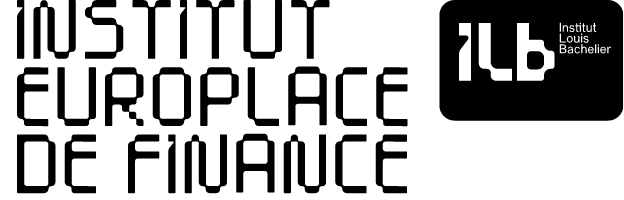
\includegraphics[height=0.62cm]{ilb.png}\hspace{0.45cm}
    
\includegraphics[height=0.62cm]{x.png}
  \end{center}
\end{frame}

\begin{frame}{Organization}
\tableofcontents
\end{frame}

% =============================================================================
\section{Introduction}

\begin{frame}{Motivation}
\small
Mean-field control is a framework for controlling a large population of interacting agents through the law of one representative agent. In discrete time,
\[
  X_{t+1}\sim P_t(\cdot\mid X_t,\mu_t,\alpha_t),
  \qquad
  \alpha_t\sim \pi_t^\theta(\cdot\mid X_t,\mu_t),
  \qquad
  \mu_t=\Law(X_t).
\]

\vspace{0.15cm}
The aim is to design policy-gradient estimators that remain model-free when the state space is not necessarily finite:
\[
  \Xc \text{ discrete or continuous},\qquad
  \mu_t\in\Pc(\Xc).
\]

\vspace{0.15cm}
The obstacle is specific to mean-field control. The policy parameter changes the sampled actions, but it also changes the population flow that is fed back into the policy, reward and transition kernel.

\vspace{0.2cm}
\scriptsize
\textbf{Where this sits.} Most numerical methods for MFC assume the model: dynamic programming, forward--backward HJB and Fokker--Planck systems, or direct differentiation through the population dynamics (Pham, Carmona, Lauri\`ere). Reinforcement learning removes that assumption, and actor--critic methods exist for MFC (Pham et al.), but a fully model-free policy gradient was available only in discrete time on a finite state space, by perturbing the logits of the population vector (Meunier et al.). This work separates that idea from the logit representation.

\vspace{0.2cm}
\small
\textbf{The central question is how to recover the missing population-flow derivative without differentiating the model.}
\end{frame}

\begin{frame}{Mean-Field Control: Two Parameter Channels}
\small
In mean-field control, the controlled law is part of the environment:
\[
  X_{t+1}^{\theta}\sim P_t(\cdot\mid X_t^\theta,\mu_t^\theta,\alpha_t^\theta),
  \qquad
  \alpha_t^\theta\sim\pi_t^\theta(\cdot\mid X_t^\theta,\mu_t^\theta),
  \qquad
  \mu_t^\theta=\Law(X_t^\theta).
\]

\[
  J(\theta)=
  \E\!\left[
    \sum_{t=0}^{T-1} r_t(X_t^\theta,\mu_t^\theta,\alpha_t^\theta)
    +g(X_T^\theta,\mu_T^\theta)
  \right].
\]

\vspace{0.15cm}
There are two ways in which $\theta$ enters the objective:
\[
\theta\longrightarrow \pi_t^\theta
\qquad\text{and}\qquad
\theta\longrightarrow \mu_t^\theta\longrightarrow
\big(\pi_t^\theta,r_t,P_t\big).
\]

\vspace{0.15cm}
The classical policy score only accounts for the first channel. The second channel is the mean-field correction.

\vspace{0.15cm}
\scriptsize
This is control, not a game. A central planner chooses one policy for the whole population and internalizes its effect on the flow, so $\mu_t^\theta$ is generated by $\theta$. In a mean-field game each agent optimizes against a flow it treats as fixed, and consistency is imposed afterwards as an equilibrium condition; there the second channel is absent by construction.
\end{frame}

\begin{frame}{Contributions}
\small
\begin{enumerate}
  \item \textbf{A perturbation at the level of measures.} Replace $\mu_t^\theta$ by the pushforward of a random transport map, so the population argument is random and its law depends on $\theta$.
  \item \textbf{A likelihood-ratio correction.} The gradient of the perturbed objective splits into the usual policy score and a population score. Neither term differentiates the kernel, the reward, or the population recursion.
  \item \textbf{A recursive sensitivity estimator.} A forward, triangular-in-time recursion for $\nabla_\theta\mu_t^\theta$, giving simulator cost linear in the horizon rather than quadratic.
  \item \textbf{Fixed-scale and adaptive algorithms}, evaluated on six benchmarks at matched simulator budgets.
\end{enumerate}

\vspace{0.3cm}
\textbf{Status, stated once and up front.}
\begin{itemize}
  \item \good{Finite state space:} complete, from the perturbation estimate through gradient convergence to the mean-square-error decomposition.
  \item \good{Continuous state space:} proved at the level of the \good{objective}.
  \item \bad{Continuous state space:} \bad{open} at the level of the \bad{gradient}. The continuous experiments run an estimator built by analogy, on exact moment charts.
\end{itemize}

\vspace{0.2cm}
\scriptsize
Full status table in the appendix. MVA submission: late August; internship continues to the end of October.
\end{frame}

% =============================================================================
\section{Background}

\begin{frame}{Why the Classical Identity Is Model-Free}
\small
In a classical Markov decision process, $X_{t+1}\sim P_t(\cdot\mid X_t,\alpha_t)$ and $\alpha_t\sim\pi_t^\theta(\cdot\mid X_t)$, the likelihood-ratio identity gives
\[
  \nabla_\theta J(\theta)
  =
  \E_\theta\!\left[
    R(\tau)
    \sum_{t=0}^{T-1}
    \nabla_\theta\log\pi_t^\theta(\alpha_t\mid X_t)
  \right].
\]

\vspace{0.2cm}
This is model-free for one specific reason: conditionally on $(X_t,\alpha_t)$, \textbf{the transition kernel does not depend on $\theta$}, so it factors out of the trajectory density before differentiation. The estimator uses sampled rewards and policy scores, and never evaluates or differentiates $P_t$.

\vspace{0.3cm}
That is exactly the property the previous slide broke: in mean-field control the kernel reads $\mu_t^\theta$, and $\mu_t^\theta$ is generated by the policy, so it does not factor out.

\vspace{0.2cm}
\centerline{\small The rest of the talk is about restoring it.}
\end{frame}

\begin{frame}{Closest Existing Construction}
\small
For finite state spaces, Meunier et al. work with strictly positive population vectors and use the logit chart
\[
  L(\mu)=\left(\log\frac{\mu(1)}{\mu(N)},\ldots,
  \log\frac{\mu(N-1)}{\mu(N)}\right)\in\R^{N-1}.
\]
They add Gaussian noise in this Euclidean chart and map back to the simplex:
\[
  Z_t^{\varepsilon,\theta}=L(\mu_t^\theta)+\varepsilon \xi_t,
  \qquad
  M_t^{\varepsilon,\theta}=\operatorname{softmax}(Z_t^{\varepsilon,\theta}).
\]

\vspace{0.15cm}
The density of $Z_t^{\varepsilon,\theta}$ gives an extra score term. Its sensitivity is the derivative of the population logits, which MF-REINFORCE estimates by an auxiliary simulation procedure.

\vspace{0.25cm}
The limitation is representation:
\[
  \text{one logit coordinate per state}.
\]
This is natural on a finite state space but has no direct analogue for a general probability measure on a continuous state space.

\vspace{0.15cm}
\textbf{The goal is to separate the perturbation idea from the particular logit representation.}
\end{frame}

% =============================================================================
\section{Methodology}

\begin{frame}{Perturbed Process and Objective}
\small
Replace the population argument by a randomized law. Let $T_t^\lambda$ be a random transport map and set
\[
  M_t^{\lambda,\theta}=T_t^\lambda\sharp\mu_t^\theta .
\]
The controlled process used by the estimator is
\[
  \alpha_t^{\lambda,\theta}\sim
  \pi_t^\theta(\cdot\mid X_t^{\lambda,\theta},M_t^{\lambda,\theta}),
  \qquad
  X_{t+1}^{\lambda,\theta}\sim
  P_t(\cdot\mid X_t^{\lambda,\theta},M_t^{\lambda,\theta},\alpha_t^{\lambda,\theta}),
\]
with perturbed objective
\[
  J^\lambda(\theta)=
  \E\!\left[
    \sum_{t=0}^{T-1}
    r_t(X_t^{\lambda,\theta},M_t^{\lambda,\theta},\alpha_t^{\lambda,\theta})
    +g(X_T^{\lambda,\theta},M_T^{\lambda,\theta})
  \right].
\]

\vspace{0.15cm}
The population argument is now random, with a density whose $\theta$-dependence can be scored. The construction then follows four steps:

\vspace{0.1cm}
\begin{enumerate}
  \item Differentiate the perturbed trajectory law by a likelihood-ratio identity.
  \item Read off a policy score and a population score.
  \item Estimate the population-flow sensitivity $D_t^\theta=\nabla_\theta\mu_t^\theta$ recursively.
  \item Send $\lambda$ to zero and control the bias--variance trade-off.
\end{enumerate}
\end{frame}

\begin{frame}{Finite State Spaces: Simplex Transport}
\small
For $\Xc=\{1,\ldots,N\}$, the population law is a vector $\mu_t^\theta\in\Delta_N$.
Let $U_t\in\R^{N-1}$ have density $\rho$, set $q_t=\varphi(U_t)\in\Delta_N^\circ$ by the softmax map, and define
\[
  M_t^{\lambda,\theta}
  =
  (1-\lambda)\mu_t^\theta+\lambda q_t,
  \qquad \lambda\in(0,1).
\]

\begin{block}{Theorem: Perturbation Estimate}
For every $\omega$,
\[
  d_{\mathrm{TV}}(M_t^{\lambda,\theta}(\omega),\mu_t^\theta)\leq\lambda.
\]
If $\Xc$ has finite diameter, then
\[
  W_1(M_t^{\lambda,\theta}(\omega),\mu_t^\theta)
  \leq \operatorname{diam}(\Xc)\lambda.
\]
\end{block}

\vspace{0.05cm}
The construction stays inside the simplex, does not require $\mu_t^\theta(i)>0$, and gives an explicit density by composing the softmax density of $q_t$ with the affine map $q\mapsto(1-\lambda)\mu_t^\theta+\lambda q$.
\end{frame}

\begin{frame}{Finite State Spaces: Gradient Structure}
\small
\begin{block}{Theorem: Policy-Gradient Formula for $J^\lambda$}
\[
  \nabla_\theta J^\lambda(\theta)
  =
  \E\!\left[\Rc_\theta^\lambda S_\theta^\lambda\right],
\]
where
\[
  S_\theta^\lambda
  =
  \sum_{t=0}^{T-1}
  \nabla_\theta\log p_t^\theta(
    \alpha_t^{\lambda,\theta}
    \mid X_t^{\lambda,\theta},M_t^{\lambda,\theta})
  -
  \frac{1-\lambda}{\lambda}
  \sum_{t=0}^{T}\sum_{k=1}^{N-1}
  H_k(q_t)\nabla_\theta\mu_t^\theta(k).
\]
\end{block}

\vspace{0.1cm}
Here $\Rc_\theta^\lambda$ is the perturbed return, $D_t^\theta(k)=\nabla_\theta\mu_t^\theta(k)$ is the population-flow sensitivity, and $H_k$ comes from the score of the perturbation density. Neither the transition kernel nor the reward is differentiated.

\vspace{0.15cm}
\begin{block}{Theorem: Convergence at Objective and Gradient Level}
Under the finite-state regularity assumptions, for every $\theta\in\Theta$ and $\lambda\in(0,1)$,
\[
  |J^\lambda(\theta)-J(\theta)|\leq C_T\lambda,
  \qquad
  \|\nabla_\theta J^\lambda(\theta)-\nabla_\theta J(\theta)\|\leq C_T^\nabla\lambda .
\]
\end{block}

\vspace{0.05cm}
The objective estimate gives consistency of optimizers by argmax-continuity: accumulation points of maximizers of $J^\lambda$ maximize $J$. So the perturbed problem is a legitimate surrogate, and its gradient is the right target.
\end{frame}

\begin{frame}{Finite State Spaces: Estimator Error}
\small
The exact sensitivity $D_t^\theta=\nabla_\theta\mu_t^\theta$ is not observed from one trajectory. The practical estimator replaces it by $\widehat D_t^{\eta,n,\theta}$, obtained from $n$ auxiliary trajectories at perturbation scale $\eta$.

\begin{block}{Proposition: Auxiliary Sensitivity Error}
For every $t=0,\ldots,T$ and $k=1,\ldots,N-1$,
\[
  \E\!\left[
  \|\widehat D_t^{\eta,n,\theta}(k)-D_t^\theta(k)\|^2
  \right]
  \leq C_T\left(\eta^2+\frac{1}{n\eta^2}\right).
\]
\end{block}

\begin{block}{Theorem: Bias and Mean-Square Error}
With $B$ main perturbed trajectories and $n$ auxiliary trajectories,
\[
  \E\|\widehat G_{\lambda,\eta,B,n}(\theta)-\nabla J(\theta)\|^2
  \leq C_T\left[
  \lambda^2
  +
  \frac{1+\lambda^{-2}}{B}
  +
  \frac1{\lambda^2}\left(\eta^2+\frac{1}{n\eta^2}\right)
  \right].
\]
\end{block}

$B$ controls the Monte Carlo variance of the main gradient estimate. $n$ controls the recursive estimate of the population-flow sensitivity.
\end{frame}

\begin{frame}{Continuous State Spaces: Charts and Perturbation}
\small
For a general state space $\mu_t^\theta$ is infinite-dimensional, and a density directly on $\Pc(\Xc)$ is not available in a useful form. So perturb coordinates instead of measures.

\begin{block}{What we call a chart}
A finite-dimensional coordinate system for the population law: an encoder $\Rc:\Pc(\Xc)\to\R^d$ and a decoder $\Gamma:\R^d\to\Pc(\Xc)$, with
\[
  z^\theta=\Rc(\mu^\theta),
  \qquad
  \bar\mu^\theta=\Gamma(z^\theta),
  \qquad
  \delta^\theta=d_\Pc(\mu^\theta,\bar\mu^\theta)\ \ \text{the representation error}.
\]
A local coordinate map in the differential-geometry sense, not a plot.
\end{block}

\vspace{-0.1cm}
Let $U_t\in\R^d$ have density $\rho$, and set $Z_t^{\lambda,\theta}=z_t^\theta+\lambda U_t$. Then
\[
  \varrho_t^{\lambda,\theta}(z)
  =
  \lambda^{-d}\rho\!\left(\frac{z-z_t^\theta}{\lambda}\right),
  \qquad
  \nabla_\theta\log \varrho_t^{\lambda,\theta}(Z_t^{\lambda,\theta})
  =
  -\frac1\lambda (D_\theta z_t^\theta)^\top\nabla\log\rho(U_t),
\]
an ordinary Euclidean score. The $\theta$-dependence is carried entirely by the translation $z_t^\theta$.

\vspace{0.1cm}
\scriptsize
Charts here: the simplex when $\Xc$ is finite, the logit map of Meunier et al., a Gaussian-mixture decoder in the theory, and the exact moment map $\mu\mapsto\E_\mu[X]$ in the experiments.
\end{frame}

\begin{frame}{Continuous State Spaces: Objective-Level Result}
\small
With the Gaussian-mixture chart $z_{K,t}^\theta=\Rc_K(\mu_t^\theta)$ and $M_{K,t}^{\lambda,\theta}=\Gamma_K(z_{K,t}^\theta+\lambda U_t)$:

\vspace{0.2cm}
\begin{block}{Theorem: Representation and Perturbation Estimate}
\[
  \E W_1(M_{K,t}^{\lambda,\theta},\mu_t^\theta)
  \leq
  \delta_{K,t}^\theta+C_{\Gamma,K}\lambda .
\]
\end{block}

\begin{block}{Theorem: Convergence of the Gaussian-Mixture Perturbed Objective}
Under stability assumptions,
\[
  |J_K^\lambda(\theta)-J(\theta)|
  \leq C_T(C_{\Gamma,K}\lambda+\delta_K^\theta).
\]
\end{block}

\vspace{0.2cm}
Two limits, kept separate: $\lambda\downarrow0$ removes the randomization, $K\to\infty$ removes the representation error. The second does not vanish with the first.

\vspace{0.15cm}
In the continuous benchmarks the chart is the exact moment map, so $\delta_K^\theta=0$ by construction and the experiments isolate the perturbation and the sensitivity recursion.
\end{frame}

\begin{frame}{Fixed-Scale Transport Algorithm}
\small
\textbf{Inputs:} policy parameter $\theta$, main scale $\lambda$, auxiliary scale $\eta$, main batch $B$, auxiliary batch $n$.

\vspace{0.15cm}
\begin{enumerate}
  \item Obtain the population argument $(\mu_t^\theta)_{t=0}^T$ from simulator rollouts or an empirical particle flow.
  \item Simulate one auxiliary batch at scale $\eta$.
  \item Recursively estimate $D_t^\theta=\nabla_\theta\mu_t^\theta$ for all $t$.
  \item Simulate $B$ perturbed main trajectories at scale $\lambda$.
  \item Combine return, policy score and population score:
  \[
    \widehat G_{\lambda,\eta,B,n}(\theta)
    =
    \frac1B\sum_{b=1}^{B}
    (R_b^\lambda-b_0)
    \left(
      \Sc_{{\rm pol},b}^{\lambda,\theta}
      +
      \widehat\Sc_{{\rm pop},b}^{\lambda,\eta,n,\theta}
    \right).
  \]
\end{enumerate}

\vspace{0.1cm}
\vspace{-0.1cm}
\begin{block}{What ``model-free'' means here, precisely}
The population argument is obtained by simulation. Exact recursions are used \textbf{only} for validation and diagnostics at frozen policies, never inside a gradient. Nothing in the estimator evaluates or differentiates $P_t$, $r_t$, or the population recursion.
\end{block}

\vspace{0.05cm}
\scriptsize
\textbf{Cost per policy update}, in simulated transitions: REINFORCE $BT$; MF-REINFORCE $BT+nT(T+1)$ with one shared auxiliary pass, against $\sim nBT^2$ as originally stated; transport $T(B_{\rm tr}+n_{\rm tr})$. The sensitivity recursion is triangular in time, so the whole flow is estimated together rather than once per time index: \textbf{linear in $T$, not quadratic}.
\end{frame}

\begin{frame}{Adaptive Transport}
\small
Fixed-scale transport requires choosing $\lambda$ and $\eta$ before training. The adaptive version keeps the estimator and moves the scales, from a bias--variance measurement taken every $100$ iterations at four nearby scale pairs.

\vspace{0.1cm}
Each checkpoint produces a debiased bias proxy and a variance proxy, combined into two balance signals $z_\lambda$ and $z_\eta$, one per scale.

\vspace{0.05cm}
\centerline{\small $z>0$: bias dominates, contract the scale. \qquad $z<0$: variance dominates, the scale may grow.}

\vspace{0.15cm}
\begin{exhibit}{Scales and balance signals over training, linear--quadratic benchmark}
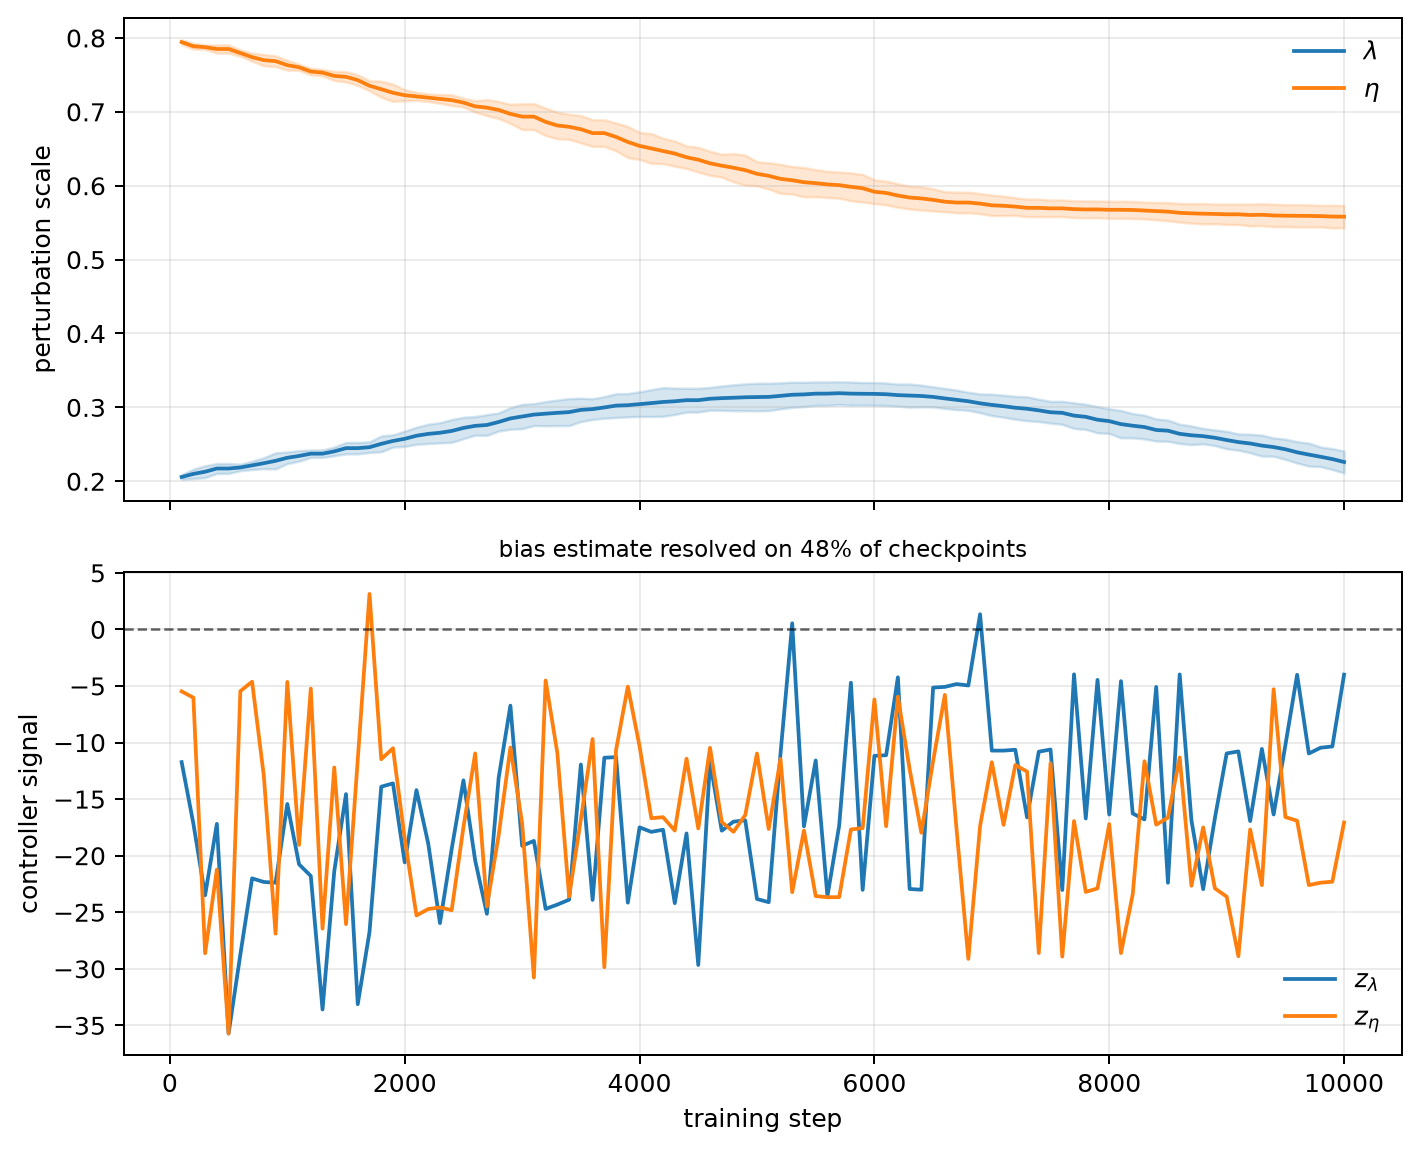
\includegraphics[width=0.40\linewidth]{lq_adaptive_schedule.png}
\end{exhibit}
\exhibitnote{Top: the two scales, five-seed mean and one standard deviation, from $(\lambda_0,\eta_0)=(0.2,0.8)$. Bottom: $z_\lambda,z_\eta$ per checkpoint.}

\vspace{0.05cm}
\scriptsize
\textbf{The diagnosis, which matters more than the controller.} It measures correctly and concludes wrongly. At four replications the debiased bias is often unresolved, the controller reads that as no bias, and contracts $\lambda$ below the calibrated grid. The score has $N-1$ coordinates and scales as $\lambda^{-1}$, so the same terminal $\lambda$ is harmless on $\Delta_2$ and damaging on $\Delta_{10}$.
\end{frame}

% =============================================================================
\section{Experiments}

\begin{frame}{Six Benchmarks, No Dominant Estimator}
\footnotesize
\textbf{Protocol.} Four estimators (REINFORCE, MF-REINFORCE, fixed-scale transport, adaptive transport) at \textbf{matched simulator budgets}, five seeds per configuration. Exact recursions and closed-form optima are used for validation only, after freezing the policy. Budgets match exactly; wall clock does not, and transport runs $2\times$ to $26\times$ slower.

\vspace{0.2cm}
\scriptsize
\begin{exhibit}{The benchmark suite and its winner, at matched simulator budget}
\begin{tabular}{llcllr}
\toprule
Benchmark & State space & $d$ & Population enters via & Best estimator & Objective \\
\midrule
Two-state ($T=5$)         & $\{0,1\}$                & 1 & reward              & Transport    & $-3.1332$ \\
Cybersecurity ($T=3$)     & $4$ states               & 3 & transition          & REINFORCE    & $-0.1517$ \\
Distribution ($T=5$)      & $\mathbb Z/10\mathbb Z$  & 9 & reward              & MF-REINFORCE & $-0.1017$ \\
Advertising ($T=5$)       & $\{0,1\}$                & 1 & transition          & MF-REINFORCE & $+0.9946$ \\
Linear--quadratic ($T=20$)& $\R$ (mean)              & 1 & dynamics and reward & Transport    & $-7.2952$ \\
Portfolio ($T=10$)        & $\R$ (mean)              & 1 & reward              & Adaptive     & $-17.193$ \\
\bottomrule
\end{tabular}
\end{exhibit}
\exhibitnote{$d$ is the number of free coordinates of the population argument. Objectives are final validation values averaged over five seeds; higher is better.}

\vspace{0.2cm}
\small
Every benchmark has a genuine mean-field coupling. Every estimator wins somewhere, and no estimator dominates the suite. The ordering is not explained by the size of the correction.
\end{frame}

\begin{frame}{Two-State Benchmark}
\scriptsize
$\Xc=\{0,1\}$, $\Ac=\{\mathrm{ST},\mathrm{MV}\}$, $P(x'\mid x,a)=\lambda_x\b1_{\{a=\mathrm{MV}\}}$ for $x'\neq x$, and
\[
  r(x,\mu)=\b1_{\{x=1\}}-\mu(1)^2-\kappa W_1(\mu,\bar\mu),
  \qquad g=r,
  \qquad
  \pi^\theta(\mathrm{ST}\mid x)=\sigma(\theta_x),\ \ \theta\in\R^2 .
\]
Interaction entirely in the reward. The policy does not read $\mu$, so the population channel is isolated: any difference between estimators is the mean-field correction and nothing else. Closed-form optimum, so both columns below are exact.

\vspace{0.15cm}
\begin{columns}[c]
\begin{column}{0.46\textwidth}
\begin{exhibit}{Validation reward, $T=2$}
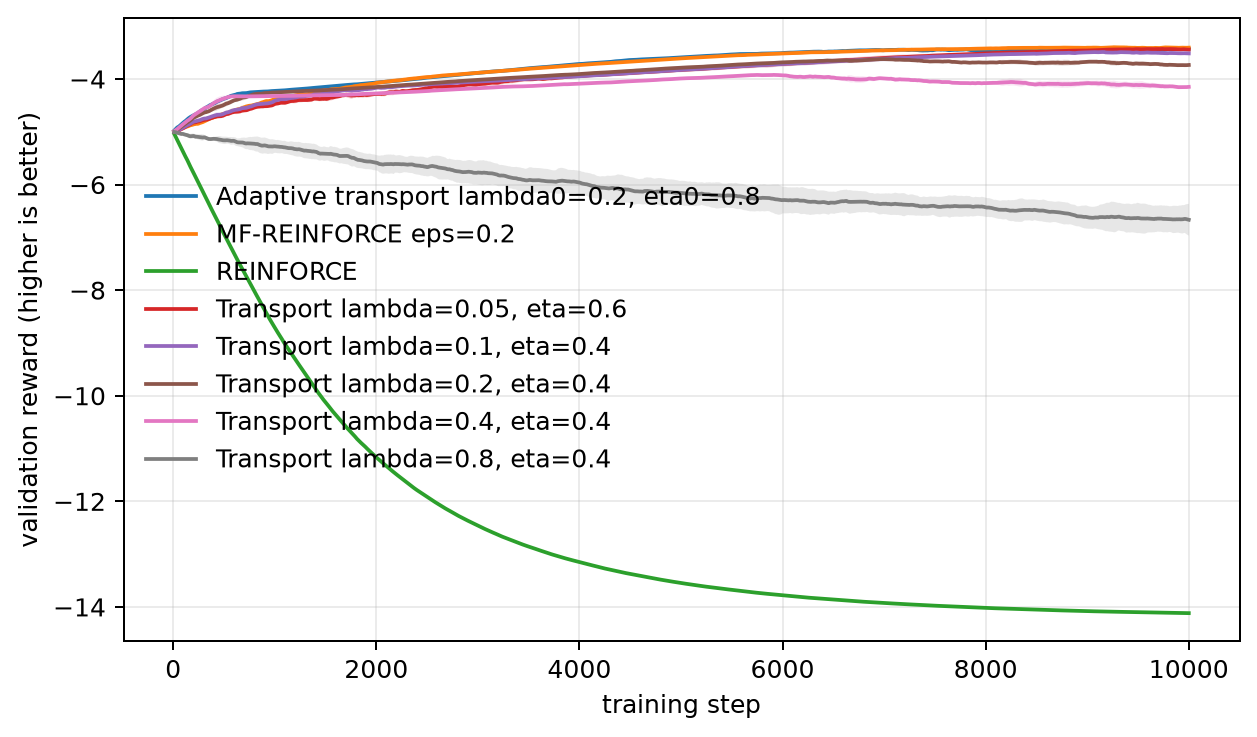
\includegraphics[width=\linewidth]{twostate_validation_T2.png}
\end{exhibit}
\end{column}
\begin{column}{0.52\textwidth}
\begin{exhibit}{Horizon comparison}
\begin{tabular}{lrrrr}
\toprule
& \multicolumn{2}{c}{$J(\theta^\star)-J(\widehat\theta)$} & \multicolumn{2}{c}{Policy error} \\
\cmidrule(lr){2-3}\cmidrule(lr){4-5}
Estimator & $T=2$ & $T=5$ & $T=2$ & $T=5$ \\
\midrule
REINFORCE    & $10.758$        & $28.870$        & $0.4694$          & $0.4691$ \\
MF-REINFORCE & $\mathbf{0.047}$& $1.565$         & $\mathbf{0.0062}$ & $0.2196$ \\
Transport    & $0.084$         & $\mathbf{0.493}$& $0.0137$          & $\mathbf{0.0347}$ \\
Adaptive     & $0.069$         & $0.756$         & $0.0100$          & $0.1160$ \\
\bottomrule
\end{tabular}
\end{exhibit}
\exhibitnote{Exact objective from $\mu_0^{\rm val}=(0.2,0.8)$: no Monte Carlo error, dispersion across five seeds only. $J(\theta^\star)=-3.360$ and $-2.640$. Policy error is $\tfrac12(e_0+e_1)$ against the optimal action probabilities.}
\end{column}
\end{columns}

\vspace{0.1cm}
\small
REINFORCE ends below its own initialization at both horizons. At $T=5$ the ordering between MF-REINFORCE and transport reverses: the auxiliary recursion is what the longer horizon stresses.
\end{frame}

\begin{frame}{Why Transport Loses Where It Loses}
\small
The correction is worth paying for only when it is both useful and resolvable. Every failure in the suite is one of those two conditions breaking, plus a cost the equal-budget rule does not charge for.

\vspace{0.2cm}
\begin{block}{1. The correction is negligible, so it is pure added variance}
\textbf{Cybersecurity} ($d=3$, population in the transition): $\varrho=+1.000$, correction fraction $0.001$. REINFORCE already computes the whole gradient. Transport pays $2.1\times$ the runtime for Monte Carlo noise. Same on the $\gamma=0$ portfolio ablation.
\end{block}

\vspace{-0.1cm}
\begin{block}{2. The correction is useful but cannot be resolved at this budget}
\textbf{Distribution planning} ($d=9$, population in the reward): nine sensitivity coordinates from $n_{\rm tr}=11$ auxiliary trajectories, so $n_{\rm tr}/d=1.2$, the worst ratio in the suite. This is consistent with the $n$ term of the MSE bound $\lambda^{-2}(\eta^2+(n\eta^2)^{-1})$ dominating, but it is an association across the suite, not yet a causal result: the frozen-policy sweep in $n$ that would settle it has not been run. MF-REINFORCE spends the same budget differently and extracts more of the same derivative.
\end{block}

\vspace{-0.1cm}
\begin{block}{3. Matched simulator budget is not matched cost}
The auxiliary recursion is cheap in transitions and expensive in arithmetic: $2\times$ to $26\times$ the REINFORCE wall clock, growing with $d$. Where REINFORCE is directionally right, it is the estimator to use.
\end{block}

\vspace{0.1cm}
\scriptsize
The adaptive controller fails for the separate reason on the previous slide. Full objective and wall-clock tables in the appendix.
\end{frame}

\begin{frame}{Targeted Advertising: Escaping a Stationary Point}
\small
State $x=1$ means customer, action $a=1$ means advertise. With $p=\mu(1)$,
\[
  P(1\mid x,a,\mu)=\min\{p+\kappa_{\rm ad}a,1\},
  \qquad
  r(x,a,\mu)=x-c_{\rm ad}a,
  \qquad g=0 .
\]
Advertising is costly, and pays only through the mean-field transition.

\vspace{-0.1cm}
\scriptsize
\begin{exhibit}{Learned advertising probability $\big(\pi(a{=}1\mid x{=}0),\ \pi(a{=}1\mid x{=}1)\big)$, by time step}
\begin{tabular}{lcccccr}
\toprule
& \multicolumn{5}{c}{(to a non-customer, to a customer)} & Customer \\
\cmidrule(lr){2-6}
Policy & $t=0$ & $t=1$ & $t=2$ & $t=3$ & $t=4$ & share at $T$ \\
\midrule
Reference $\widehat q$ & $(1.00,1.00)$ & $(1.00,1.00)$ & $(1.00,1.00)$ & $(1.00,1.00)$ & $(0.64,0.64)$ & --- \\
REINFORCE    & $(0.00,0.00)$ & $(0.00,0.00)$ & $(0.00,0.00)$ & $(0.00,0.00)$ & $(0.00,0.00)$ & $0.200$ \\
MF-REINFORCE & $(1.00,1.00)$ & $(1.00,1.00)$ & $(0.02,0.01)$ & $(0.00,0.00)$ & $(0.00,0.00)$ & $0.603$ \\
Transport    & $(1.00,0.00)$ & $(1.00,0.00)$ & $(1.00,0.00)$ & $(1.00,0.00)$ & $(1.00,0.00)$ & $0.738$ \\
\bottomrule
\end{tabular}
\end{exhibit}
\exhibitnote{Each entry is a pair of probabilities of playing $a=1$ (advertise), the first conditional on the agent being a non-customer ($x=0$), the second on the agent being a customer ($x=1$). \textbf{Best seed of each estimator}, so the rows show what each method can reach, not what it reaches on average. Last column: customer share $\mu_T(1)$ from the validation law $\mu_0(1)=0.2$.}

\vspace{0.15cm}
\small
Never advertising is a stationary point of the detached objective, and REINFORCE stays trapped on it at every seed. The population-aware estimators produce escaping runs, into structurally different policies: MF-REINFORCE truncates in time, transport targets by state. Transport escapes on most seeds, not on all: at $\lambda=0.1$, three of five reach the targeted policy and two remain near the plateau.
\end{frame}

\begin{frame}{Continuous-State Benchmarks}
\scriptsize
\textbf{Linear--quadratic.} $\pi_t^\theta(\cdot\mid x,m)=\Nc(\theta_t^1x+\theta_t^2\bar m_t,\tau^2)$, $X_{t+1}=aX_t+b\alpha_t+c\bar m_t+\sigma\varepsilon_{t+1}$, quadratic costs, Riccati optimum. \quad
\textbf{Portfolio.} $X_{t+1}=s_tX_t+\alpha_tR_{t+1}$, $r=-\gamma\mu^2$, $g(x,\mu)=x-\chi(x-\mu)^2$, $\mu_t=\E[X_t]$, $\gamma=2$.

\vspace{0.1cm}
\alert{These are exact moment-chart experiments, not a general continuous-state theorem.} In both, the perturbed argument is the population mean, so the chart is exact, one-dimensional, and $\delta_K^\theta=0$. No Gaussian mixture is fitted anywhere. The estimator is built by analogy with the finite-state case; its guarantees here are an extrapolation.

\vspace{0.1cm}
\begin{exhibit}{Mean validation objective against training iteration, five seeds}
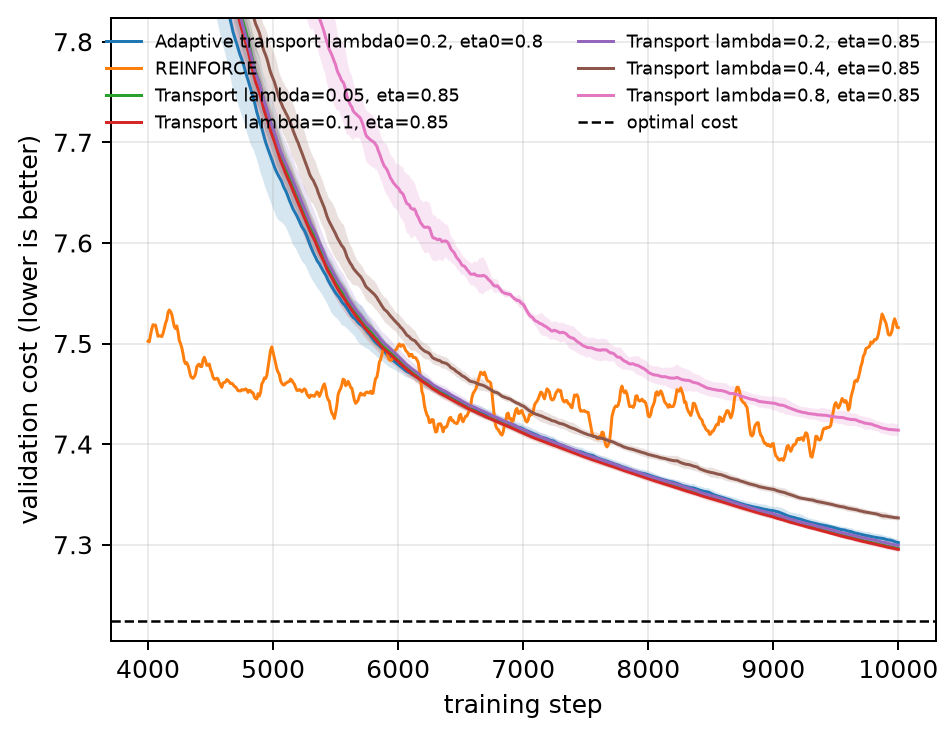
\includegraphics[height=3.1cm]{lq_convergence_validation.png}
\hspace{0.4cm}
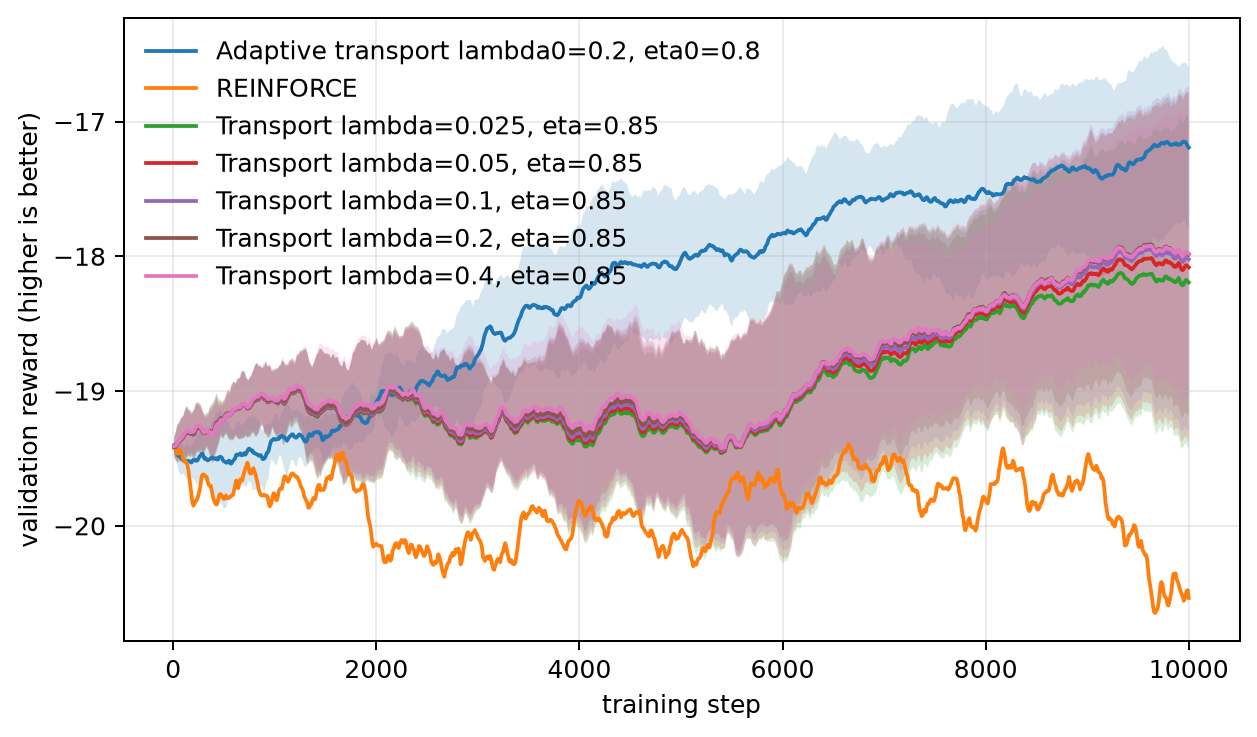
\includegraphics[height=3.1cm]{portfolio_validation_T10.png}
\end{exhibit}
\exhibitnote{Left: linear--quadratic, $T=20$, cost convention. Right: mean--variance portfolio, $T=10$.}

\vspace{0.05cm}
\begin{exhibit}{Final objective and gap to the closed-form optimum}
\begin{tabular}{lrrrr}
\toprule
& \multicolumn{2}{c}{Linear--quadratic ($T=20$)} & \multicolumn{2}{c}{Portfolio ($T=10$)} \\
\cmidrule(lr){2-3}\cmidrule(lr){4-5}
Method & Objective & Gap & Objective & Gap \\
\midrule
Closed-form optimum & $-7.2238$          & $0$              & $-13.133$           & $0$ \\
REINFORCE           & $-7.5157$          & $0.292$          & $-20.535$           & $7.402$ \\
Transport           & $\mathbf{-7.2952}$ & $\mathbf{0.072}$ & $-17.980$           & $4.847$ \\
Adaptive            & $-7.3021$          & $0.078$          & $\mathbf{-17.193}$  & $\mathbf{4.060}$ \\
\bottomrule
\end{tabular}
\end{exhibit}
\exhibitnote{Gap is $|J(\widehat\theta)-J(\theta^\star)|$; $\theta^\star$ from the Riccati recursion and from the closed-form affine optimum. Both terms exact.}
\end{frame}

\begin{frame}{Validating the Theory}
\small
Four predictions of the analysis are testable from the saved artifacts. None of these quantities is available to the training algorithms.

\vspace{0.2cm}
\scriptsize
\begin{exhibit}{Predictions, the quantity that tests each, and the outcome}
\begin{tabular}{lll}
\toprule
Prediction & Measured quantity & Outcome \\
\midrule
$\TV(M_t^{\lambda,\theta},\mu_t^\theta)\leq\lambda$
  & $\max_t \TV/\lambda$ along the learned flow
  & holds at $445/445$, ratio up to $1.00$ \\
$|J^\lambda-J|\leq C_T\lambda$
  & bias$/\lambda^2$ over a $16\times$ range of $\lambda$
  & constant to $0.1\%$ (LQ), $7\%$ (portfolio) \\
$\E[\widehat G]=\nabla_\theta J^\lambda$, oracle $D$
  & $\chi^2$ test, $50$ replications
  & $p=1.000,\,1.000,\,0.996$ at $\lambda\leq0.2$ \\
$\mathrm{MSE}=\mathrm{bias}^2+\mathrm{dispersion}$
  & the identity, run by run
  & closes to the $(R-1)/R$ factor \\
\bottomrule
\end{tabular}
\end{exhibit}
\exhibitnote{The first is measured on every finite-state transport run, the others on the linear--quadratic and portfolio benchmarks, the only two exposing a closed-form gradient oracle.}

\vspace{0.25cm}
\small
\begin{itemize}
  \item The perturbation bound is attained: the ratio reaches $1.00$ on distribution planning.
  \item The objective bias is $O(\lambda^2)$, one order better than the theorem guarantees.
  \item Unbiasedness holds over the calibrated range and fails at $\lambda=0.8$, outside it.
  \item On the portfolio the test is inconclusive rather than passed: signal-to-noise $0.02$ per replication.
\end{itemize}
\end{frame}

\begin{frame}{The Diagnostic: Correction Alignment}
\small
At frozen policies, compare the full gradient with the gradient obtained by detaching the population flow from the computational graph:
\[
  G_{\rm full}=\nabla_\theta J(\theta,\mu^\theta),
  \qquad
  G_{\rm det}=\nabla_\theta J(\theta,\mu)\big|_{\mu=\mu^\theta},
  \qquad
  \varrho=\frac{\langle G_{\rm full},G_{\rm det}\rangle}{\|G_{\rm full}\|\,\|G_{\rm det}\|}.
\]
$G_{\rm det}$ is what REINFORCE estimates. Adam is invariant to positive rescaling, so what matters is the component of the correction orthogonal to $G_{\rm det}$, not its size.

\vspace{0.15cm}
\scriptsize
\begin{exhibit}{Correction alignment at reference policies, and the observed ordering}
\begin{tabular}{lrll}
\toprule
Benchmark & $\varrho$ & Geometry & REINFORCE \\
\midrule
Two-state            & $-1.000$ & opposed            & fails \\
Targeted advertising & $-0.921$ & opposed            & fails \\
Portfolio            & $-0.196$ & nearly orthogonal  & fails \\
Distribution         & $+0.092$ & nearly orthogonal  & fails \\
\midrule
Linear--quadratic    & $+0.985$ & nearly parallel    & competitive \\
Cybersecurity        & $+1.000$ & correction negligible & best \\
\bottomrule
\end{tabular}
\end{exhibit}
\exhibitnote{Mean over five independent reference policies, each obtained by running REINFORCE for $300$ iterations from the benchmark initialization.}

\vspace{0.05cm}
\centerline{\small\alert{Evaluation-only. Not part of the model-free estimator: it needs a differentiable evaluation path.}}

\vspace{0.2cm}
\small
Two separated groups, nothing between $0.092$ and $0.985$. What carries the information is the distance from $+1$, not the sign of $\varrho$.

\vspace{0.1cm}
Alignment predicts whether REINFORCE is directionally competitive. It does not rank the estimators.
\end{frame}

\begin{frame}{Controlled Pair: Switching the Population Channel Off}
\small
On the portfolio benchmark the coefficient $\gamma$ multiplies the only reward term that depends explicitly on the population, so it can be switched off with the dynamics held fixed.

\vspace{0.15cm}
At $\gamma=0$ the terminal reward depends on the population only through the centred variable $x-\mu$, and at the consistent law
\[
  \partial_\mu\,\E\!\left[-\chi(X-\mu)^2\right]
  =
  2\chi\left(\E[X]-\mu\right)
  =
  0 ,
\]
so the mean-field correction is exactly zero for any value of the terminal risk parameter $\chi$.

\vspace{0.15cm}
\scriptsize
\begin{exhibit}{Portfolio benchmark with the population channel switched off and on}
\begin{tabular}{lccl}
\toprule
 & $\|G_{\rm full}\|$ vs $\|G_{\rm det}\|$ & $\varrho$ & Training outcome \\
\midrule
$\gamma=0$ & $0.083$ vs $0.083$ & $+1.000$ & REINFORCE recovers $42\%$ of the range; transport ends below its start \\
$\gamma=2$ & $1.357$ vs $0.083$ & $-0.196$ & transport and adaptive beat REINFORCE by about $2.5$ \\
\bottomrule
\end{tabular}
\end{exhibit}
\exhibitnote{Only $\gamma$ changes between the two rows. The dynamics, the estimators, the budgets and the seeds are identical.}

\vspace{0.25cm}
\small
Same dynamics, same estimators, opposite ordering. The causal evidence behind the alignment story; the previous table is an association across six points.

\vspace{0.1cm}
At $\gamma=0$ the correction measured on the estimator is $83\%$ of the gradient, all of it Monte Carlo noise. Magnitude is the wrong diagnostic.
\end{frame}

% =============================================================================
\section{Discussion}

\begin{frame}{Strengths and Limitations}
\small
\textbf{Strengths.}
\begin{itemize}
  \item \textbf{Measure-level perturbation:} works for discrete and continuous state spaces (with finite representations).
  \item \textbf{Simplex transport:} defined on the boundary of the simplex, where the logit chart is not.
  \item \textbf{Recursive sensitivity:} simulator cost linear in the horizon rather than quadratic.
  \item \textbf{Testable before it is paid for:} the alignment diagnostic costs two AD passes and no training grid, wherever a differentiable evaluation path exists.
  \item \textbf{Predictions checked against the runs:} four of them, on the recorded artifacts.
\end{itemize}

\vspace{0.3cm}
\textbf{Limitations.}
\begin{itemize}
  \item \textbf{Continuous gradient-level theory is open:} the continuous estimator is an extrapolation.
  \item \textbf{Matched simulator budget is not matched cost:} $2\times$ to $26\times$ slower in wall clock.
  \item \textbf{The auxiliary estimate can dominate the variance:} an association across the suite, not yet causal.
  \item \textbf{The adaptive controller is the weakest component:} it reads unresolved bias as no bias.
  \item \textbf{The evidence is bounded by the design:} two oracle benchmarks, five seeds.
\end{itemize}
\end{frame}

\begin{frame}{Extensions}
\small
\textbf{Continuous theory.} Gradient-level convergence, the policy-gradient formula, and MSE bounds carrying the representation error $\delta_K^\theta$. The main open item.

\vspace{0.25cm}
\textbf{Actor--critic estimator.} Replace full returns by advantages, to reduce the variance amplified by the $\lambda^{-1}$ score.

\vspace{0.25cm}
\textbf{Auxiliary budget allocation.} Immediate test: distribution planning at the same budget, split moved from $(549,11)$ to $(200,360)$, for $1.9\times$ the cost per step.

\vspace{0.25cm}
\textbf{Adaptive controller.} A floor on $\lambda$ and a dimension-aware variance target.

\vspace{0.25cm}
\textbf{Richer law statistics.} Fourier modes in Kuramoto-type synchronization: a two-dimensional chart.

\vspace{0.25cm}
\textbf{Extended and non-exchangeable MFC.} Coefficients reading the joint law of $(X_t,\alpha_t)$, and graphon limits where the population argument is indexed by vertex type.

\vspace{0.3cm}
\scriptsize
The internship runs to the end of October.
\end{frame}

\begin{frame}{Conclusion}
\small
\[
\begin{array}{c}
  \text{discrete-time MFC}
  \longrightarrow
  \text{randomized population argument}
  \longrightarrow
  \text{policy score + population score}\\[2pt]
  \longrightarrow
  \text{recursive sensitivity estimator}
  \longrightarrow
  \text{bias--variance control}.
\end{array}
\]

\vspace{0.2cm}
\begin{itemize}
  \item The finite-state transport estimator is theoretically complete through MSE bounds.
  \item The continuous-state construction is proved at objective level and implemented on exact moment charts.
  \item Transport is valuable when the mean-field correction changes the optimization direction enough to compensate its variance.
  \item Where a differentiable evaluation path exists, the alignment diagnostic gives a cheap indication, before any training grid, of whether REINFORCE is directionally reliable. It is evaluation-only, and separate from the model-free estimator itself.
\end{itemize}
\end{frame}

% =============================================================================
\appendix
\AtBeginSection[]{}
\section{Appendix}

\begin{frame}{Appendix}
\small
\begin{columns}[T]
\begin{column}{0.49\textwidth}
\textbf{Theory}
\begin{itemize}\scriptsize
  \item What is proved, implemented, and open
  \item Why REINFORCE is biased in MFC
  \item What we call a chart
  \item Finite-state perturbation density and score
  \item Recursive sensitivity estimator
  \item Assumptions behind the finite-state results
  \item Proof architecture
  \item Continuous Gaussian-mixture chart
  \item Comparison with MF-REINFORCE
  \item Complexity comparison
\end{itemize}

\vspace{0.2cm}
\textbf{Open directions}
\begin{itemize}\scriptsize
  \item The actor--critic extension
  \item A benchmark with a two-dimensional law statistic
\end{itemize}
\end{column}
\begin{column}{0.49\textwidth}
\textbf{Experiments}
\begin{itemize}\scriptsize
  \item Protocol, budgets and reproducibility
  \item Cybersecurity and distribution planning results
  \item The bias--variance trade-off, measured
  \item Wall-clock cost
  \item Auxiliary budget per coordinate
  \item Reallocation control
  \item Calibration grid in $(\lambda,\eta)$
  \item Perturbation bound and objective bias
  \item Perturbation bias versus optimization error
  \item Objective summary, all six benchmarks
  \item Adaptive scales and controller diagnosis
  \item Cybersecurity and distribution planning models
  \item Targeted advertising, escaping the plateau
  \item Two-state learned population flows
  \item Distribution planning terminal law
  \item Particle-flow robustness
\end{itemize}
\end{column}
\end{columns}
\end{frame}

% -----------------------------------------------------------------------------
% Theory
% -----------------------------------------------------------------------------

\begin{frame}{Appendix: What Is Proved, What Is Implemented, What Is Open}
\scriptsize
\begin{exhibit}{Status of each contribution, by state space}
\begin{tabular}{lll}
\toprule
Result & Finite state space & Continuous state space \\
\midrule
Perturbation estimate ($\TV$, $W_1$)   & \good{proved} & \good{proved} \\
Density and score of the perturbation  & \good{proved} & \good{proved} \\
Convergence of the perturbed objective & \good{proved} & \good{proved} \\
Consistency of optimizers              & \good{proved} & \good{proved} \\
\midrule
Gradient-level convergence             & \good{proved} & \bad{open} \\
Policy-gradient representation         & \good{proved} & \bad{open} \\
Estimator of the flow sensitivity      & \good{proved} & \bad{no general theorem} \\
Bias and mean-square-error bounds      & \good{proved} & \bad{open} \\
\midrule
Algorithms and benchmarks    & \multicolumn{2}{l}{implemented; $640$ runs over six benchmarks} \\
Four theoretical predictions & \multicolumn{2}{l}{measured; three confirmed, unbiasedness for $\lambda\leq0.2$} \\
Alignment diagnostic         & \multicolumn{2}{l}{empirical: six benchmarks and one controlled pair} \\
\bottomrule
\end{tabular}
\end{exhibit}

\vspace{0.15cm}
\small
The continuous-state construction is established at the level of the objective and open at the level of the gradient. The continuous experiments therefore run an estimator built by analogy with the finite-state case, on exact moment charts where the representation error is zero by construction.

\vspace{0.1cm}
Closing that gap is the main open item. The internship runs to the end of October.
\end{frame}

\begin{frame}{Appendix: Why REINFORCE Is Biased in Mean-Field Control}
\small
Write the objective with the population flow as an explicit second argument, $J(\theta)=\Jc(\theta,\mu^\theta)$. The total derivative is
\[
  \nabla_\theta J(\theta)
  =
  \underbrace{\partial_\theta\Jc(\theta,\mu)\big|_{\mu=\mu^\theta}}_{G_{\rm det},\ \text{what REINFORCE estimates}}
  +
  \underbrace{\partial_\mu\Jc(\theta,\mu^\theta)\big[\nabla_\theta\mu^\theta\big]}_{\text{the mean-field correction}} .
\]

\vspace{0.15cm}
In a classical MDP the second term is absent: conditionally on $(X_t,\alpha_t)$, the transition kernel does not depend on $\theta$. In mean-field control the population law is generated by the policy itself, so $\theta$ reaches the reward, the kernel and the policy argument a second time through $\mu_t^\theta$.

\vspace{0.15cm}
Two consequences visible in the experiments:
\begin{itemize}
  \item REINFORCE converges to a stationary point of the detached objective, which need not be stationary for $J$. Targeted advertising is exactly this: never advertising is stationary for $G_{\rm det}$ and REINFORCE cannot leave it.
  \item When the correction opposes $G_{\rm det}$, REINFORCE ascends a descent direction. On two-state it ends at $-31.51$ from an initialization of $-4.53$.
\end{itemize}

\vspace{0.15cm}
The difficulty is that $\nabla_\theta\mu_t^\theta$ is a derivative of the model. The construction recovers it by a likelihood ratio rather than by differentiating anything.
\end{frame}

\begin{frame}{Appendix: What We Call a Chart}
\small
A chart is a finite-dimensional coordinate system for the population law, in the differential-geometry sense of a local coordinate map. It is a pair
\[
  \Rc:\Pc(\Xc)\to\R^{q}\ \ \text{(encoder)},
  \qquad
  \Gamma:\R^{q}\to\Pc(\Xc)\ \ \text{(decoder)},
\]
with $z^\theta=\Rc(\mu^\theta)$, $\bar\mu^\theta=\Gamma(z^\theta)$ and representation error $\delta^\theta=d_\Pc(\mu^\theta,\bar\mu^\theta)$.

\vspace{0.15cm}
\scriptsize
\begin{exhibit}{The charts appearing in this work}
\begin{tabular}{llcl}
\toprule
Chart & Coordinates $z$ & $q$ & Representation error \\
\midrule
Simplex (ours, finite $\Xc$)   & the probability vector $\mu$ & $N-1$ & $0$, exact \\
Logit (Meunier et al.)         & $\log(\mu(i)/\mu(N))$        & $N-1$ & $0$, but needs $\mu(i)>0$ \\
Gaussian mixture (theory)      & weights, means, Cholesky     & $q_K$ & $\delta_K^\theta>0$ in general \\
Moment (continuous experiments)& $\E_\mu[X]$                  & $1$   & $0$ by construction \\
\bottomrule
\end{tabular}
\end{exhibit}

\vspace{0.1cm}
\small
The point of the framework is that the perturbation is defined on the measure and the score is read in the chart, so the two are separable. The chart must satisfy three things: it is finite-dimensional, its coordinates are differentiable in $\theta$, and it retains the functionals of the law that the dynamics, the reward and the policy actually read.

\vspace{0.1cm}
An exact chart is one with $\delta^\theta=0$. Both continuous benchmarks are exact because the coefficients read the mean and nothing else, which is why they test the perturbation and the sensitivity recursion with no mixture-fitting error superposed.
\end{frame}

\begin{frame}{Appendix: Finite-State Perturbation Density and Score}
\small
For $\mu\in\Delta_N$ and $q\in\Delta_N^\circ$,
\[
  M^\lambda=(1-\lambda)\mu+\lambda q .
\]
Let $U\in\R^{N-1}$ have density $\rho$ and $q=\varphi(U)$ the softmax map, so $q$ has a smooth density on the relative interior of the simplex. The density of $M^\lambda$ follows by the affine change of variables $q\mapsto(1-\lambda)\mu+\lambda q$, and its score is
\[
  \nabla_\theta\log f_t^{\lambda,\theta}(m)
  =
  -\frac{1-\lambda}{\lambda}
  \sum_{k=1}^{N-1}H_k(q)\,\nabla_\theta\mu_t^\theta(k),
  \qquad
  q=\frac{m-(1-\lambda)\mu_t^\theta}{\lambda}.
\]

\vspace{0.15cm}
Three features of this expression:
\begin{itemize}
  \item The $\theta$-dependence is carried entirely by the translation $\mu_t^\theta$, exactly as $z^\theta$ carries it in the continuous chart.
  \item $H_k$ depends only on $\rho$ and the softmax map, so it is known in closed form and costs nothing.
  \item The prefactor $\lambda^{-1}$ is the source of the bias--variance trade-off: shrinking $\lambda$ reduces the perturbation bias and inflates this score.
\end{itemize}

\vspace{0.15cm}
The construction stays inside $\Delta_N$ for every $\lambda\in(0,1)$ and does not require $\mu_t^\theta(i)>0$, which is what the logit chart needs.

\vspace{0.15cm}
\scriptsize
\textbf{What $\rho$ is in the experiments.} Isotropic Gaussian pushed through the softmax: $q_t=\operatorname{softmax}(U_t^{(1)},\ldots,U_t^{(N-1)},0)$ with $U_t\sim\Nc(0,I_{N-1})$, so $q_t$ is logistic-normal on $\Delta_N^\circ$. On $\Delta_2$ this reduces to $q_t=(\sigma(U_t),1-\sigma(U_t))$ with $U_t\sim\Nc(0,1)$. The theory allows any smooth $\rho$; no ablation over that choice was run.
\end{frame}

\begin{frame}{Appendix: Recursive Sensitivity Estimator}
\small
The auxiliary process runs at the second scale $\eta$, with
\[
  \bar M_s^{\eta,\theta}=(1-\eta)\mu_s^\theta+\eta\bar q_s .
\]
For $k<N$,
\[
  D_t^\theta(k)
  =
  \lim_{\eta\downarrow0}
  \E\!\left[
    \b1_{\{\bar X_t^{\eta,\theta}=k\}}
    \sum_{s=0}^{t-1}
    \left(
      \Psi_s^{\eta,\theta}
      -
      \frac{1-\eta}{\eta}
      \sum_{\ell=1}^{N-1}H_\ell(\bar q_s)D_s^\theta(\ell)
    \right)
  \right].
\]

\vspace{0.1cm}
$D_0^\theta=0$ since $\mu_0$ does not depend on $\theta$, so the system is triangular in time and can be solved forward.

\vspace{0.15cm}
This is where the cost saving comes from. The sensitivity at time $t$ uses only $D_s^\theta$ for $s<t$ and the same auxiliary batch, so one shared forward pass of $n$ trajectories gives the whole flow $(D_t^\theta)_{t=0}^T$: cost $T(B+n)$ rather than $nT(T+1)$ per main trajectory.

\vspace{0.15cm}
\begin{block}{Proposition: auxiliary sensitivity error}
\[
  \E\big\|\widehat D_t^{\eta,n,\theta}(k)-D_t^\theta(k)\big\|^2
  \leq
  C_T\Big(\eta^2+\frac{1}{n\eta^2}\Big).
\]
\end{block}
\scriptsize
The $\eta^2$ term is the bias of the finite-$\eta$ target, the $(n\eta^2)^{-1}$ term the likelihood-ratio variance. This is the one prediction the saved artifacts cannot split into its two parts, since that needs a sweep in $n$ at a frozen policy.
\end{frame}

\begin{frame}{Appendix: Assumptions Behind the Finite-State Results}
\footnotesize
\textbf{Uniform regularity} (objective-level results). There are constants $L_K,L_R,L_g$ and bounds $\bar R,\bar g$ such that for all $\theta,t,i$ and $m,m'\in\Delta_N$,
\[
  \TV\big(K_t^\theta(\cdot\mid i,m),K_t^\theta(\cdot\mid i,m')\big)\leq L_K\TV(m,m'),
\]
\[
  |R_t^\theta(i,m)-R_t^\theta(i,m')|\leq L_R\TV(m,m'),
  \qquad
  |g(i,m)-g(i,m')|\leq L_g\TV(m,m'),
\]
with $|R_t^\theta|\leq\bar R$ and $|g|\leq\bar g$. In words: the averaged kernel and the reward are Lipschitz in the population argument in total variation, uniformly in the policy parameter, and the rewards are bounded.

\vspace{0.2cm}
\textbf{Smoothness of the averaged dynamics} (gradient-level results). $(\theta,m)\mapsto K_t^\theta(\cdot\mid i,m)$ and $(\theta,m)\mapsto R_t^\theta(i,m)$ are $C^1$ in both arguments, uniformly in $t,i$, and their first derivatives are Lipschitz in $m$ and in the direction, with all first derivatives uniformly bounded.

\vspace{0.2cm}
\textbf{Differentiability and integrability} (policy-gradient formula). Differentiation under the expectation is justified: the policy is $C^1$ in $\theta$ with integrable score, and the perturbation density is $C^1$ with integrable score.

\vspace{0.2cm}
\textbf{Continuous case, additionally.} Regularity of the Gaussian-mixture decoder, $\E W_1(\Gamma_K(z+\lambda U),\Gamma_K(z))\leq C_{\Gamma,K}\lambda$; and Wasserstein stability of the controlled dynamics. Non-degeneracy is imposed on the representation: weights bounded away from zero, covariances uniformly positive definite, and a fixed component ordering, since $\Gamma_K$ is not injective under permutations.

\vspace{0.15cm}
\scriptsize
All \textbf{four finite-state} benchmarks satisfy these assumptions: finite $\Xc$ and $\Ac$, bounded rewards, and kernels affine or Lipschitz in $\mu$. The two continuous-state benchmarks are covered only by the objective-level results, and their estimator is an extrapolation.
\end{frame}

\begin{frame}{Appendix: Proof Architecture}
\footnotesize
Each result feeds the next; nothing is proved by differentiating the model.

\vspace{0.15cm}
\begin{enumerate}
  \item \textbf{Perturbation estimate.} $M_t^{\lambda,\theta}=(1-\lambda)\mu_t^\theta+\lambda q_t$ gives $\TV(M_t^{\lambda,\theta},\mu_t^\theta)=\lambda\TV(q_t,\mu_t^\theta)\leq\lambda$ pathwise, and $W_1\leq\operatorname{diam}(\Xc)\lambda$ on a bounded state space.
  \item \textbf{Stability of the state marginal.} A finite-horizon induction on the dual representation of total variation gives $\TV(\nu_t^{\lambda,\theta},\mu_t^\theta)\leq L_K\lambda t$: the perturbation injected at each step accumulates at most linearly.
  \item \textbf{Objective convergence.} Summing the reward Lipschitz bounds along the horizon gives $|J^\lambda(\theta)-J(\theta)|\leq C_T\lambda$, uniformly in $\theta$.
  \item \textbf{Consistency of optimizers.} Uniform convergence plus an argmax-continuity argument: accumulation points of maximizers of $J^\lambda$ maximize $J$. This is what makes the perturbed problem a legitimate surrogate.
  \item \textbf{Gradient-level convergence.} The same induction run on the differentiated marginal gives $\|E_t^{\lambda,\theta}[h]-D_t^\theta[h]\|_1\leq C_T^D\lambda$, then $\|\nabla J^\lambda-\nabla J\|\leq C_T^\nabla\lambda$.
  \item \textbf{Policy-gradient formula.} The augmented trajectory density factorizes into the policy, the perturbation density and the kernel; only the first two depend on $\theta$, so differentiating under the expectation gives the two scores and never touches the kernel.
  \item \textbf{Unbiasedness and MSE.} Under oracle $D$ the estimator is exactly unbiased for $\nabla J^\lambda$. Conditioning on the auxiliary batch isolates the plug-in error, and the conditional variance decomposition assembles
  \[
    \E\|\widehat G-\nabla J\|^2\leq C_T\Big[\lambda^2+\tfrac{1+\lambda^{-2}}{B}+\tfrac1{\lambda^2}\big(\eta^2+\tfrac1{n\eta^2}\big)\Big].
  \]
\end{enumerate}
\end{frame}

\begin{frame}{Appendix: Continuous Gaussian-Mixture Chart}
\small
\[
  \Gc_K=
  \left\{\sum_{k=1}^{K}w_k\Nc(m_k,\Sigma_k)
  : w\in\Delta_K^\circ,\ m_k\in\R^d,\ \Sigma_k\in\Sc_{++}^d\right\}.
\]
Unconstrained coordinates, of dimension $q_K=(K-1)+Kd+K\tfrac{d(d+1)}2$:
\[
  z=(\beta,m_1,\ldots,m_K,s_1,\ldots,s_K)\in\R^{q_K},
  \qquad
  \Gamma_K:\R^{q_K}\to\Gc_K,
\]
with $w(\beta)$ the logistic parametrization and $\Sigma(s_k)=L(s_k)L(s_k)^\top$ a Cholesky factor whose diagonal is exponentiated. $\Gamma_K$ plays the role the softmax plays on the simplex: perturb freely in $\R^{q_K}$, land in a valid probability measure.

\vspace{0.15cm}
\[
  z_{K,t}^\theta=\Rc_K(\mu_t^\theta),
  \qquad
  Z_{K,t}^{\lambda,\theta}=z_{K,t}^\theta+\lambda U_t,
  \qquad
  M_{K,t}^{\lambda,\theta}=\Gamma_K(Z_{K,t}^{\lambda,\theta}).
\]
For $U_t\sim\Nc(0,\Xi)$,
\[
  \nabla_\theta\log\varrho_{K,t}^{\lambda,\theta}(Z_{K,t}^{\lambda,\theta})
  =
  \lambda^{-1}(D_\theta z_{K,t}^{\theta})^\top\Xi^{-1}U_t .
\]

\vspace{0.15cm}
\scriptsize
The random measure $M_{K,t}^{\lambda,\theta}$ never needs a density on $\Pc(\R^d)$, which would be awkward since $\Gamma_K$ is not injective under permutations. The Euclidean variable is kept in the augmented trajectory and every likelihood ratio runs against Lebesgue measure on $\R^{q_K}$. Because the mixture coordinates have different scales, a block-diagonal $\Xi$ over weight, mean and covariance blocks is preferable in practice.

\vspace{0.1cm}
Nothing in the argument uses the mixture structure. Any chart with a decoder, a randomization and a differentiable $z^\theta$ gives the same density, the same score and the same objective estimate.
\end{frame}

\begin{frame}{Appendix: Comparison with MF-REINFORCE}
\footnotesize
\begin{exhibit}{The two model-free constructions, side by side}
\begin{tabular}{lll}
\toprule
 & MF-REINFORCE (Meunier et al.) & Transport (this work) \\
\midrule
Perturbation lives on & the logits $L(\mu)\in\R^{N-1}$ & the measure itself \\
Perturbed argument & $\operatorname{softmax}(L(\mu_t^\theta)+\varepsilon\xi_t)$ & $(1-\lambda)\mu_t^\theta+\lambda q_t$ \\
Requires $\mu_t^\theta(i)>0$ & yes & no \\
State space & finite only & finite or continuous, via a chart \\
Sensitivity estimated & separately per time index & once, by a triangular recursion \\
Simulator cost & $BT+nT(T+1)$ & $T(B_{\rm tr}+n_{\rm tr})$ \\
Scale parameters & $\varepsilon$ & $\lambda$ (main), $\eta$ (auxiliary) \\
\bottomrule
\end{tabular}
\end{exhibit}

\vspace{0.15cm}
\small
The original Algorithm 1 performs the auxiliary pass inside the loop over the $B$ main trajectories, giving $BT+B\,nT(T+1)\sim nBT^2$. The logit gradient is a property of the policy and the flow rather than of an individual trajectory, so our implementation estimates it once per update and shares it. The equal-budget comparison uses the cheaper of the two, which is the conservative choice, since it is the budget every other estimator must match.

\vspace{0.1cm}
$\varepsilon$ is not retuned here. We use the best values reported in the reference study, $\varepsilon=0.2,\ 1.0,\ 2.0$ on two-state, cybersecurity and distribution; advertising is not in that grid and uses $\varepsilon=1.0$.
\end{frame}

% -----------------------------------------------------------------------------
% Experiments
% -----------------------------------------------------------------------------

\begin{frame}{Appendix: Protocol, Budgets and Reproducibility}
\footnotesize
\begin{itemize}
  \item \textbf{Configurations.} A configuration is a benchmark, horizon, algorithm, flow mode, perturbation scales and budget. Five independent seeds each. In a paired comparison the seed fixes the policy initialization, the training initial laws, the Monte Carlo samples and the validation schedule.
  \item \textbf{Grids.} Two-state is the calibration experiment, over $\lambda\in\{0.05,0.1,0.2,0.4,0.8\}$ against $\eta\in\{0.4,0.6,0.85,0.95\}$. After it, $\eta=0.85$ is fixed everywhere else and the $\lambda$-grid is reduced.
  \item \textbf{Adaptive.} Initialized at $(\lambda_0,\eta_0)=(0.2,0.8)$ on every benchmark, diagnostics every $100$ iterations from $R=4$ replications. A scale moves only on a resolved bias estimate or a sign change in the direction test.
  \item \textbf{Training.} Adam. Validation every ten iterations, without exploration noise where an exact population recursion exists. Training randomizes the initial law; validation uses a fixed law or a fixed grid. Exact objectives, dynamic-programming references and closed-form optima are used only after freezing the parameters.
  \item \textbf{Policies.} Two hidden layers of width $32$ on the finite-state benchmarks; a directly parametrized affine policy on the continuous ones.
  \item \textbf{Diagnostics.} Evaluation-only, at saved policies, never entering a training update: bias, dispersion, MSE, cosine alignment with the oracle, and the size of the correction.
  \item \textbf{Scale.} $640$ runs, roughly $94$ hours of single-core compute, on one machine with an NVIDIA RTX A4000, executed on the CPU device since a step is dominated by simulation rather than by parameter updates. Every figure and table is regenerated from the saved artifacts.
\end{itemize}
\end{frame}

\begin{frame}{Appendix: Complexity Comparison}
\small
The unit is one simulated transition per policy update.

\begin{exhibit}{Simulator cost per policy update}
\begin{tabular}{ll}
\toprule
Estimator & Cost per policy update \\
\midrule
REINFORCE & $C_{\rm RF}=BT$ \\
MF-REINFORCE (ours, shared auxiliary pass) & $C_{\rm MF}=BT+nT(T+1)$ \\
MF-REINFORCE (as in Meunier et al., Alg.~1) & $C_{\rm MF}=BT+B\,nT(T+1)\sim nBT^2$ \\
Transport & $C_{\rm tr}=T(B_{\rm tr}+n_{\rm tr})$ \\
\bottomrule
\end{tabular}
\end{exhibit}
\exhibitnote{Counted in simulated transitions. $B$ main trajectories, $n$ auxiliary trajectories, horizon $T$.}

\vspace{0.15cm}
The transport estimator uses one shared auxiliary forward pass. The sensitivity recursion is triangular in time, so the whole sensitivity flow is estimated together instead of separately for each time index.
\end{frame}

\begin{frame}{Appendix: Wall-Clock Cost}
\scriptsize
\begin{exhibit}{Simulator budget and wall clock per run, five-seed mean}
\begin{tabular}{llrrr}
\toprule
Benchmark & Estimator & Simulator budget & Wall clock (s) & Ratio to REINFORCE \\
\midrule
Two-state & REINFORCE & $1\,300$ & $48$ & $1.0\times$ \\
 & MF-REINFORCE & $1\,300$ & $252$ & $5.3\times$ \\
 & Transport & $1\,300$ & $200$ & $4.2\times$ \\
\midrule
Cybersecurity & REINFORCE & $612$ & $532$ & $1.0\times$ \\
 & MF-REINFORCE & $612$ & $1\,199$ & $2.3\times$ \\
 & Transport & $612$ & $1\,122$ & $2.1\times$ \\
\midrule
Distribution planning & REINFORCE & $2\,800$ & $263$ & $1.0\times$ \\
 & MF-REINFORCE & $2\,800$ & $6\,622$ & $25.1\times$ \\
 & Transport & $2\,800$ & $6\,802$ & $25.8\times$ \\
\midrule
Targeted advertising & REINFORCE & $1\,300$ & $146$ & $1.0\times$ \\
 & MF-REINFORCE & $1\,300$ & $463$ & $3.2\times$ \\
 & Transport & $1\,300$ & $372$ & $2.6\times$ \\
\midrule
Linear--quadratic & REINFORCE & $4\,420$ & $113$ & $1.0\times$ \\
 & Transport & $4\,420$ & $1\,069$ & $9.5\times$ \\
\midrule
Portfolio & REINFORCE & $5\,110$ & $59$ & $1.0\times$ \\
 & Transport & $5\,110$ & $352$ & $5.9\times$ \\
\bottomrule
\end{tabular}
\end{exhibit}
\exhibitnote{The budget is matched by construction on every benchmark. For transport the slowest entry of the grid is reported. The ratio tracks the dimension of the population argument: the auxiliary recursion is cheap in transitions and expensive in arithmetic.}
\end{frame}

\begin{frame}{Appendix: Auxiliary Budget per Coordinate}
\scriptsize
\begin{exhibit}{Split of the matched budget between main and auxiliary trajectories}
\begin{tabular}{llrrrrr}
\toprule
Benchmark & Argument & $d$ & $B_{\rm tr}$ & $n_{\rm tr}$ & $n_{\rm tr}/d$ & Budget \\
\midrule
Two-state & $\Delta_2$ & 1 & 248 & 12 & $12.0$ & $1\,300$ \\
Cybersecurity & $\Delta_4$ & 3 & 184 & 20 & $6.7$ & $612$ \\
Distribution & $\Delta_{10}$ & 9 & 549 & 11 & $\mathbf{1.2}$ & $2\,800$ \\
Advertising & $\Delta_2$ & 1 & 248 & 12 & $12.0$ & $1\,300$ \\
LQ & mean & 1 & 201 & 20 & $20.0$ & $4\,420$ \\
Portfolio & mean & 1 & 311 & 200 & $200.0$ & $5\,110$ \\
\bottomrule
\end{tabular}
\end{exhibit}
\exhibitnote{$d$ is the number of free coordinates of the population argument. The equal-budget rule constrains $T(B_{\rm tr}+n_{\rm tr})$ but not the split.}

\vspace{0.15cm}
\small
The ratio spans more than two orders of magnitude, and distribution planning is the only benchmark where it falls close to one sample per coordinate. It is also the finite-state benchmark on which transport loses most heavily. That is an association across six points, not a result.

\vspace{0.1cm}
The portfolio row is the counterexample that keeps it from being sufficient: $200$ auxiliary trajectories for a one-dimensional argument, and still an optimization error of at least $4.97$.
\end{frame}

\begin{frame}{Appendix: Reallocation Control}
\small
The experiment that would turn the association above into a result: on distribution planning, move the split from $(B_{\rm tr},n_{\rm tr})=(549,11)$ to $(200,360)$. The matched budget $T(B_{\rm tr}+n_{\rm tr})=2\,800$ is unchanged and the auxiliary estimate rises to $40$ trajectories per coordinate. The measured cost is $1.9\times$ in seconds per step rather than the $33\times$ the sample increase would suggest, since the recursion is applied to the batch at once. This has not been run.

\vspace{0.2cm}
\scriptsize
\begin{exhibit}{Negative control, already recorded: same reallocation where the estimate is already resolved}
\begin{tabular}{llrrrrr}
\toprule
Benchmark & $\lambda$ & $B_{\rm tr}$ & $n_{\rm tr}$ & $n_{\rm tr}/d$ & Iterations & Objective \\
\midrule
Targeted advertising & $0.1$ & 248 & 12 & $12.0$ & $10\,000$ & $0.9795\pm0.0089$ \\
 &  & 100 & 160 & $160.0$ & $10\,000$ & $0.9734\pm0.0079$ \\
\bottomrule
\end{tabular}
\end{exhibit}
\exhibitnote{Same estimator, scales, simulator budget and iteration count; only the split differs. Five seeds. Higher is better.}

\vspace{0.15cm}
\small
On advertising the auxiliary estimate is already resolved at the default split, so the hypothesis predicts the reallocation should do nothing. It moves the objective by less than one standard deviation, which is what is observed. The control is consistent with the hypothesis; the test itself is still outstanding.
\end{frame}

\begin{frame}{Appendix: Calibration Grid in $(\lambda,\eta)$}
\small
\begin{exhibit}{Two-state at $T=5$, exact flow: final validation objective, five-seed mean}
\begin{tabular}{lrrrr}
\toprule
& \multicolumn{4}{c}{Auxiliary scale $\eta$} \\
\cmidrule(lr){2-5}
$\lambda$ & $0.4$ & $0.6$ & $0.85$ & $0.95$ \\
\midrule
$0.05$ & $-4.369$ & $-3.686$ & $-3.228$ & $-3.198$ \\
$0.1$ & $-4.287$ & $-3.510$ & $-3.154$ & $\mathbf{-3.133}$ \\
$0.2$ & $-4.381$ & $-3.811$ & $-3.603$ & $-3.614$ \\
$0.4$ & $-5.312$ & $-4.979$ & $-4.855$ & $-4.874$ \\
$0.8$ & $-6.003$ & $-9.129$ & $-9.836$ & $-9.877$ \\
\bottomrule
\end{tabular}
\end{exhibit}
\exhibitnote{Higher is better; the exact optimum is $-2.640$. This grid fixes $\eta=0.85$ for the remaining benchmarks.}

\vspace{0.15cm}
\small
The optimum is interior in $\lambda$, which is the bias--variance trade-off of the main perturbation showing up directly in the training outcome.

\vspace{0.1cm}
In $\eta$ the objective increases over the whole range whenever $\lambda\leq0.1$, and peaks at $\eta=0.85$ for $\lambda\in\{0.2,0.4\}$: the auxiliary estimator wants a large radius, because at these sample sizes the $(n\eta^2)^{-1}$ variance term dominates its $O(\eta)$ bias. The ordering reverses only at $\lambda=0.8$, where the run is already dominated by perturbation bias.
\end{frame}

\begin{frame}{Appendix: Perturbation Bound and Objective Bias}
\scriptsize
\begin{columns}[T]
\begin{column}{0.47\textwidth}
\begin{exhibit}{$\TV$ bound on the finite-state runs}
\begin{tabular}{lrrr}
\toprule
Benchmark & Cfg. & Pts & $\max_t\TV/\lambda$ \\
\midrule
Two-state & 80 & 400 & $0.800$ \\
Cybersecurity & 3 & 15 & $0.843$ \\
Distribution & 3 & 15 & $1.000$ \\
Advertising & 3 & 15 & $0.800$ \\
\midrule
Total & $89$ & $445$ & $445/445$ hold \\
\bottomrule
\end{tabular}
\end{exhibit}
\end{column}
\begin{column}{0.51\textwidth}
\begin{exhibit}{Perturbation bias of the optimal value}
\begin{tabular}{llrrr}
\toprule
Benchmark & $\lambda$ & $|J^\lambda_\star-J_\star|$ & $/\lambda$ & $/\lambda^2$ \\
\midrule
LQ & $0.05$ & $0.2754$ & $5.51$ & $110.17$ \\
 & $0.1$ & $1.1015$ & $11.01$ & $110.15$ \\
 & $0.2$ & $4.4047$ & $22.02$ & $110.12$ \\
 & $0.4$ & $17.6126$ & $44.03$ & $110.08$ \\
 & $0.8$ & $70.4299$ & $88.04$ & $110.05$ \\
\midrule
Portfolio & $0.025$ & $0.0308$ & $1.23$ & $49.34$ \\
 & $0.05$ & $0.1231$ & $2.46$ & $49.23$ \\
 & $0.1$ & $0.4887$ & $4.89$ & $48.87$ \\
 & $0.2$ & $1.9171$ & $9.59$ & $47.93$ \\
 & $0.4$ & $7.3465$ & $18.37$ & $45.92$ \\
\bottomrule
\end{tabular}
\end{exhibit}
\end{column}
\end{columns}

\vspace{0.15cm}
\small
Left: the largest $\TV(M_t^{\lambda,\theta},\mu_t^\theta)$ along the learned flow of every finite-state transport run, against $\lambda$. The bound holds everywhere and is attained on distribution planning, so the perturbation is neither degenerate nor larger than the theory allows.

\vspace{0.1cm}
Right: the theorem bounds this by $C_T\lambda$, so the fourth column must stay bounded and the fifth would diverge if the rate were exactly linear. It does not. Both objectives are quadratic in the population argument, so the linear term of the expansion vanishes at the optimum and the bias is $O(\lambda^2)$. The measurement recovers that exponent rather than contradicting the theorem.
\end{frame}

\begin{frame}{Appendix: The Bias--Variance Trade-Off, Measured}
\scriptsize
\begin{exhibit}{Gradient diagnostics, linear--quadratic benchmark, $R=50$ replications at $8\,192$ particles}
\begin{tabular}{lrrrrrrr}
\toprule
$\lambda$ & $\|\nabla J^\lambda-\nabla J\|$ & $/\lambda^2$ & $\|\E[\widehat G]-\nabla J^\lambda\|$ & $p$ & Dispersion & $d\cdot\mathrm{MSE}$ & $\cos$ \\
\midrule
$0.05$ & $0.0030$ & $1.18$ & $0.0421$ & $1.000$ & $0.5926$ & $0.3500$ & $0.941$ \\
$0.1$  & $0.0115$ & $1.15$ & $0.0480$ & $1.000$ & $0.6151$ & $0.3763$ & $0.914$ \\
$0.2$  & $0.0433$ & $1.08$ & $0.0702$ & $0.996$ & $0.7234$ & $0.5224$ & $0.892$ \\
$0.4$  & $0.1562$ & $0.98$ & $0.1963$ & $0.123$ & $1.2290$ & $1.5232$ & $0.742$ \\
$0.8$  & $0.5899$ & $0.92$ & $0.9565$ & $0.000$ & $4.7778$ & $23.2859$ & $0.643$ \\
\bottomrule
\end{tabular}
\end{exhibit}
\exhibitnote{Column 2 is the perturbation bias of the gradient against the closed-form oracle, column 3 divides it by $\lambda^2$. Column 4 is the bias of the estimator with respect to the perturbed gradient it targets, column 5 the $\chi^2$ $p$-value that this bias is zero. Column 6 is the replication dispersion, column 7 the mean-square error scaled by the parameter dimension, column 8 the cosine alignment with the oracle.}

\vspace{0.1cm}
\small
This is the trade-off of the MSE theorem, read off a single table. At $\lambda=0.05$ the dispersion is $0.59$ against a squared bias of $0.0018$, so the error is essentially all variance. At $\lambda=0.8$ the dispersion has grown to $4.78$ and the bias to $0.96$, and both terms deteriorate together while the alignment falls monotonically from $0.94$ to $0.64$.

\vspace{0.05cm}
Column 3 is constant to within $1\%$: the gradient bias scales as $\lambda^2$, matching the objective-level measurement by an independent route. Column 7 equals the sum of the squares of columns 4 and 6 to the $(R-1)/R$ factor, which is the MSE decomposition verified run by run.
\end{frame}

\begin{frame}{Appendix: Perturbation Bias versus Optimization Error}
\scriptsize
\begin{exhibit}{Linear--quadratic at $T=20$, cost convention, lower is better, $J(\theta^\star)=7.224$}
\begin{tabular}{lrrrr}
\toprule
$\lambda$ & $J^\lambda(\theta_\lambda^\star)$ & Perturbation bias & Optimization error & Optimality gap \\
& & $|J^\lambda(\theta_\lambda^\star)-J(\theta^\star)|$ & $|J^\lambda(\widehat\theta_\lambda)-J^\lambda(\theta_\lambda^\star)|$ & $|J(\widehat\theta_\lambda)-J(\theta^\star)|$ \\
\midrule
$0.05$ & $7.499$ & $0.275$ & $0.0733\pm0.0021$ & $0.0723\pm0.0021$ \\
$0.1$ & $8.325$ & $1.101$ & $0.0756\pm0.0025$ & $\mathbf{0.0715\pm0.0023}$ \\
$0.2$ & $11.628$ & $4.405$ & $0.0916\pm0.0029$ & $0.0754\pm0.0021$ \\
$0.4$ & $24.836$ & $17.613$ & $0.1631\pm0.0068$ & $0.1028\pm0.0028$ \\
$0.8$ & $77.654$ & $70.430$ & $0.4246\pm0.0211$ & $0.1901\pm0.0059$ \\
\midrule
Adaptive & --- & --- & --- & $0.0783\pm0.0030$ \\
REINFORCE & --- & --- & --- & $0.2920\pm0.0010$ \\
\bottomrule
\end{tabular}
\end{exhibit}
\exhibitnote{All entries from closed-form expressions with no Monte Carlo error, so the dispersion is entirely across the five seeds.}

\vspace{0.1cm}
\small
The residual of a fixed-scale run splits into a property of the problem the estimator targets and a property of the run. The perturbation bias carries no seed dispersion. The optimization error is the only part a better estimator could remove. The last column is not the sum of the other two, since a policy optimized for $J^\lambda$ need not be displaced from $\theta^\star$ by the full bias of the objective.

\vspace{0.1cm}
The portfolio benchmark falls out the other way: perturbation bias at most $7.35$ across the grid, optimization error never below $4.97$. There the limitation is estimator variance, not perturbation bias.
\end{frame}

\begin{frame}{Appendix: Objective Summary, All Six Benchmarks}
\scriptsize
\begin{exhibit}{Final validation objective, five-seed mean, higher is better}
\begin{tabular}{lrrrr}
\toprule
Benchmark & REINFORCE & MF-RF & Transport & Adaptive \\
\midrule
Two-state ($T=5$) & $-31.5104$ & $-4.2053$ & $\mathbf{-3.1332}$ & $-3.3960$ \\
Cybersecurity ($T=3$) & $\mathbf{-0.1517}$ & $-0.1524$ & $-0.1544$ & $-0.1602$ \\
Distribution ($T=5$) & $-0.2616$ & $\mathbf{-0.1017}$ & $-0.2421$ & $-0.5596$ \\
Advertising ($T=5$) & $0.9688$ & $\mathbf{0.9946}$ & $0.9795$ & $0.9727$ \\
Linear--quadratic ($T=20$) & $-7.5157$ & --- & $\mathbf{-7.2952}$ & $-7.3021$ \\
Portfolio ($T=10$) & $-20.535$ & --- & $-17.980$ & $\mathbf{-17.193}$ \\
\bottomrule
\end{tabular}
\end{exhibit}
\exhibitnote{At the headline horizon and flow mode of each benchmark. MF-REINFORCE is finite-state only. For transport, the best entry of the calibration grid.}

\vspace{0.15cm}
\small
Three regimes. Where the population channel carries the sign of the useful direction, an estimator that differentiates the flow wins by far more than the seed dispersion, by an order of magnitude on two-state. Where the correction helps but the auxiliary estimate is unresolved, the logit estimator extracts more of it. Where the correction vanishes, REINFORCE is best and the whole spread is under $6\%$ of the objective.
\end{frame}

\begin{frame}{Appendix: Adaptive Scales and Controller Diagnosis}
\scriptsize
\begin{exhibit}{Scales reached from $(\lambda_0,\eta_0)=(0.2,0.8)$ on every benchmark}
\begin{tabular}{llrrrr}
\toprule
Benchmark & Flow & $\lambda$ after training & $\eta$ after training & Best fixed $\lambda$ & Resolved bias \\
\midrule
Two-state & exact & $0.039\pm0.002$ & $0.365\pm0.023$ & $0.1$ & $66\%$ \\
Cybersecurity & exact & $0.026\pm0.000$ & $0.214\pm0.005$ & $0.4$ & $68\%$ \\
Distribution & exact & $0.025\pm0.000$ & $0.201\pm0.001$ & $0.4$ & $72\%$ \\
Advertising & exact & $0.040\pm0.004$ & $0.361\pm0.024$ & $0.1$ & $64\%$ \\
LQ & exact & $0.226\pm0.015$ & $0.558\pm0.015$ & $0.1$ & $48\%$ \\
Portfolio & exact & $0.597\pm0.027$ & $0.336\pm0.040$ & $0.4$ & $47\%$ \\
\bottomrule
\end{tabular}
\end{exhibit}
\exhibitnote{Last column: the fraction of checkpoints at which the debiased bias estimate was resolved and the main scale was therefore allowed to move.}

\vspace{0.15cm}
\small
The terminal scale alone does not separate the failures from the successes: $\lambda$ lands at $0.025$--$0.040$ on all four finite-state benchmarks, below $0.05$, the smallest calibrated scale, yet the outcome is acceptable on two-state and advertising and bad on cybersecurity and distribution.

\vspace{0.1cm}
What separates them is the dimension of the population argument, $\Delta_2$ against $\Delta_4$ and $\Delta_{10}$. The perturbation score has $N-1$ coordinates and scales as $\lambda^{-1}$, so contracting $\lambda$ inflates a variance that grows with the dimension, and the same terminal $\lambda$ is harmless on $\Delta_2$ and damaging on $\Delta_{10}$.

\vspace{0.1cm}
The controller is not failing to measure: the bias is resolved at $68\%$ and $72\%$ of checkpoints on the two failures, the highest rates in the suite, against $48\%$ on the linear--quadratic benchmark where the outcome is good. It measures a small bias correctly and draws the wrong conclusion, because the balance rule weighs bias against variance without accounting for the $\lambda^{-1}$ growth of the score. The fix is a floor on $\lambda$ and a dimension-aware target.
\end{frame}

\begin{frame}{Appendix: Cybersecurity and Distribution Planning Results}
\small
\textbf{Cybersecurity} ($4$ states, $d=3$, population in the transition). Defended/undefended $\times$ infected/susceptible, population-dependent infection intensities.
\par\vspace{0.2cm}
\textbf{Distribution planning} ($\mathbb Z/10\mathbb Z$, $d=9$, population in the reward). Move mass on a torus towards a target law. The largest population argument in the suite.

\vspace{0.25cm}
\scriptsize
\begin{exhibit}{Final objective and wall clock at matched simulator budget}
\begin{tabular}{lrrrr}
\toprule
& \multicolumn{2}{c}{Cybersecurity ($T=3$)} & \multicolumn{2}{c}{Distribution ($T=5$)} \\
\cmidrule(lr){2-3}\cmidrule(lr){4-5}
Estimator & Objective & Wall clock & Objective & Wall clock \\
\midrule
REINFORCE    & $\mathbf{-0.1517}$ & $532$\,s  & $-0.2616$          & $263$\,s \\
MF-REINFORCE & $-0.1524$          & $1199$\,s & $\mathbf{-0.1017}$ & $6622$\,s \\
Transport    & $-0.1544$          & $1122$\,s & $-0.2421$          & $6802$\,s \\
Adaptive     & $-0.1602$          & $1026$\,s & $-0.5596$          & $5975$\,s \\
\bottomrule
\end{tabular}
\end{exhibit}
\exhibitnote{Objectives are final validation values over five seeds, higher is better; wall clock is the full training run on one machine.}

\vspace{0.2cm}
\small
Two different failure modes.
\end{frame}

\begin{frame}{Appendix: Cybersecurity and Distribution Planning Models}
\scriptsize
\textbf{Cybersecurity.} $\Xc=\{\mathrm{DI},\mathrm{DS},\mathrm{UI},\mathrm{US}\}$, defended/undefended $\times$ infected/susceptible; the action switches protection status. Infection intensities depend on the population:
\[
  \iota_D(\mu)=v_Hq_{\rm inf}^D+\beta_{DD}\mu(\mathrm{DI})+\beta_{UD}\mu(\mathrm{UI}),
  \qquad
  \iota_U(\mu)=v_Hq_{\rm inf}^U+\beta_{UU}\mu(\mathrm{UI})+\beta_{DU}\mu(\mathrm{DI}),
\]
\[
  r_{\Delta t}(x,a,\mu)=-\Delta t\left[k_D\b1_{\{x\in\{\mathrm{DI},\mathrm{DS}\}\}}+k_I\b1_{\{x\in\{\mathrm{DI},\mathrm{UI}\}\}}\right].
\]
The population enters through the transition. $d=3$. The winning behaviour is to stop defending and accept the undefended equilibrium, and the correction is negligible: $\varrho=+1.000$ to six decimals, correction fraction $0.001$.

\vspace{0.3cm}
\textbf{Distribution planning.} $\Xc=\mathbb Z/10\mathbb Z$, $\Ac=\{-1,0,+1\}$, $P(x'\mid x,a,\mu)=\b1_{\{x'=x+a\ ({\rm mod}\ 10)\}}$, with
\[
  \mu_{\rm target}=(0.02,0.04,0.09,0.16,0.19,0.19,0.16,0.09,0.04,0.02),
\]
\[
  r(x,a,\mu)=-c_{\rm mov}|a|-\|\mu-\mu_{\rm target}\|_2^2,
  \qquad
  g(x,\mu)=-\|\mu-\mu_{\rm target}\|_2^2 .
\]
The population enters through the reward. Nine free coordinates, the largest population argument in the suite, and the worst auxiliary ratio: $n_{\rm tr}/d=1.2$.

\vspace{0.25cm}
\textbf{Targeted advertising.} $\Xc=\Ac=\{0,1\}$; with $p=\mu(1)$, $P(1\mid x,a,\mu)=\min\{p+\kappa_{\rm ad}a,1\}$, $r(x,a,\mu)=x-c_{\rm ad}a$, $g=0$. The population enters through the transition, and $\mu$ evolves by a one-dimensional deterministic recursion. Based on the model of Motte and Pham.
\end{frame}

\begin{frame}{Appendix: Targeted Advertising, Escaping the Plateau}
\small
\begin{exhibit}{Mean validation reward against training iteration, five seeds}
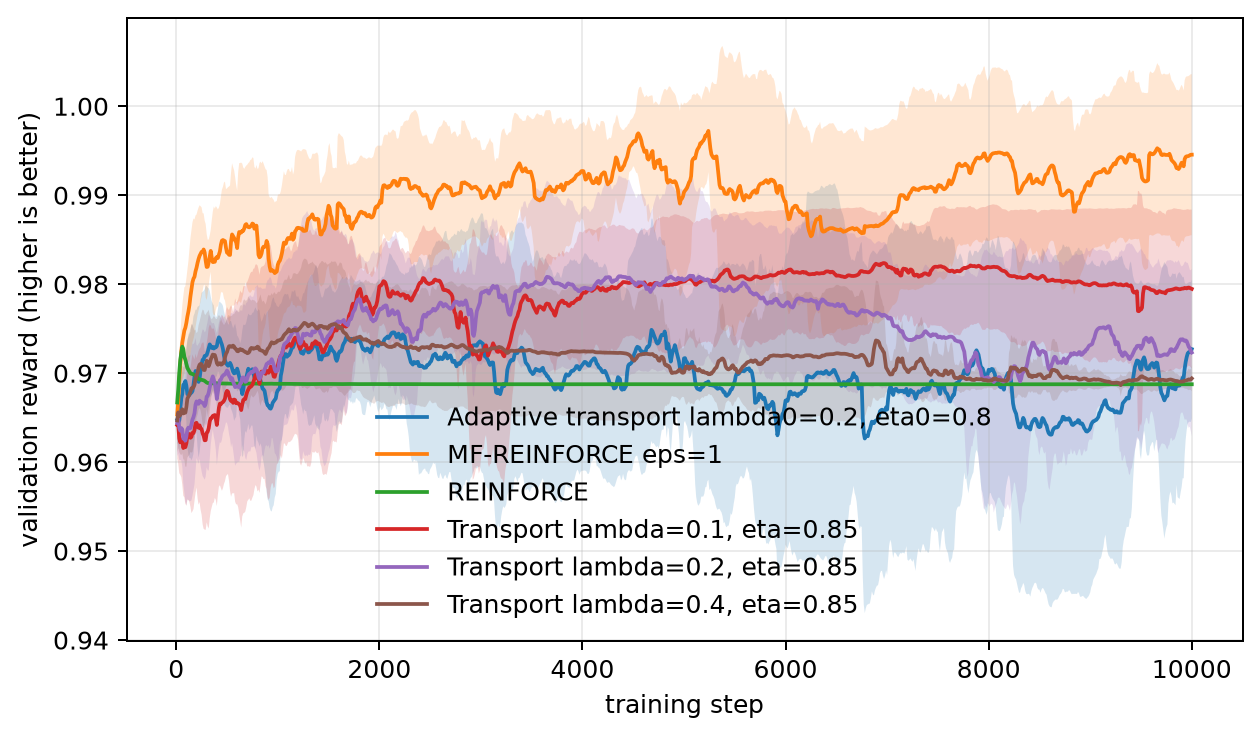
\includegraphics[width=0.60\linewidth]{advertising_validation_T5.png}
\end{exhibit}
\exhibitnote{REINFORCE is the flat line at $0.9688$: it reaches the never-advertise plateau within a few hundred iterations and stays there at every seed. The population-aware estimators produce escaping runs; transport escapes on most seeds, not on all.}

\vspace{0.1cm}
\small
The reward scale compresses everything: the whole spread between a policy that never advertises and one that nearly matches the reference is under $3\%$ of the objective.

\vspace{0.1cm}
The seed dispersion is bimodal rather than diffuse. At $\lambda=0.1$, three seeds reach the state-targeted policy and two remain near the REINFORCE plateau, so the mean advertising probability of $0.31$ describes no individual run. Transport escapes the plateau on most seeds, not on every one.
\end{frame}

\begin{frame}{Appendix: Two-State Learned Population Flows}
\small
\begin{exhibit}{Learned flow $t\mapsto\mu_t(0)$ by estimator, two-state at $T=5$}
\scriptsize
\begin{tabular}{cc}
\textbf{REINFORCE} & \textbf{MF-REINFORCE} \\[2pt]
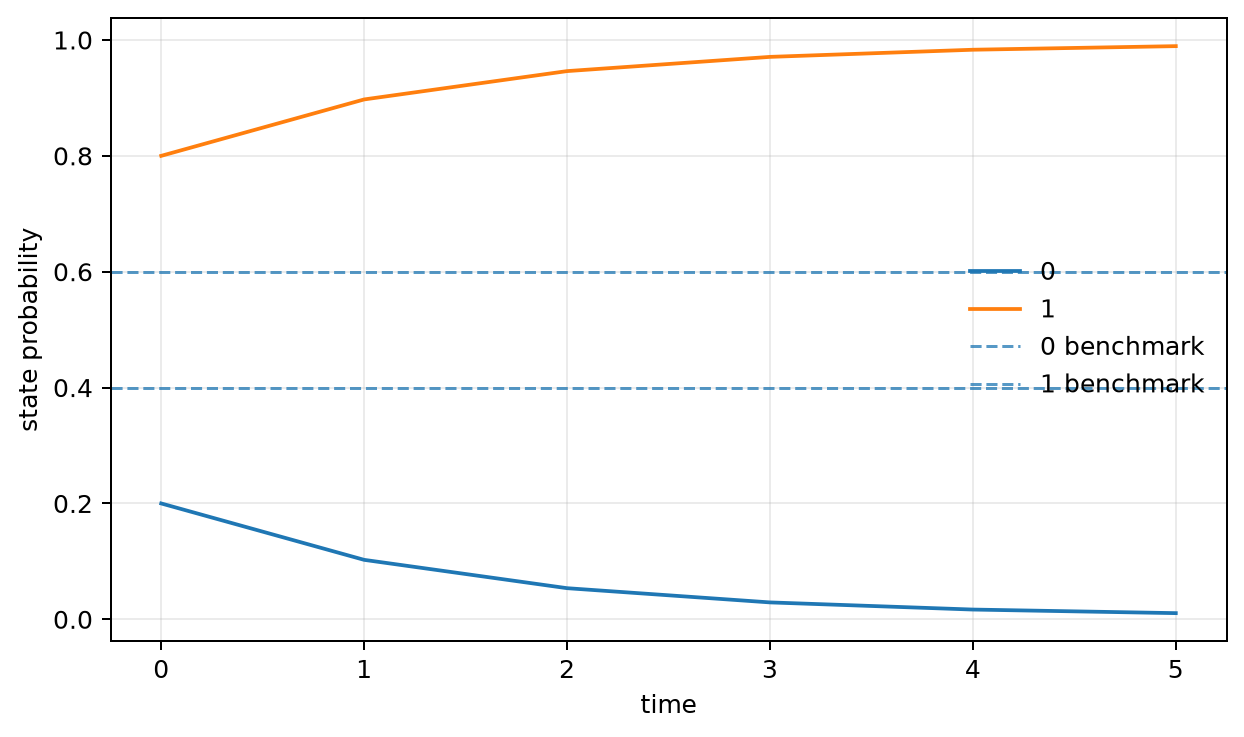
\includegraphics[width=0.34\linewidth]{twostate_flow_reinforce.png} &
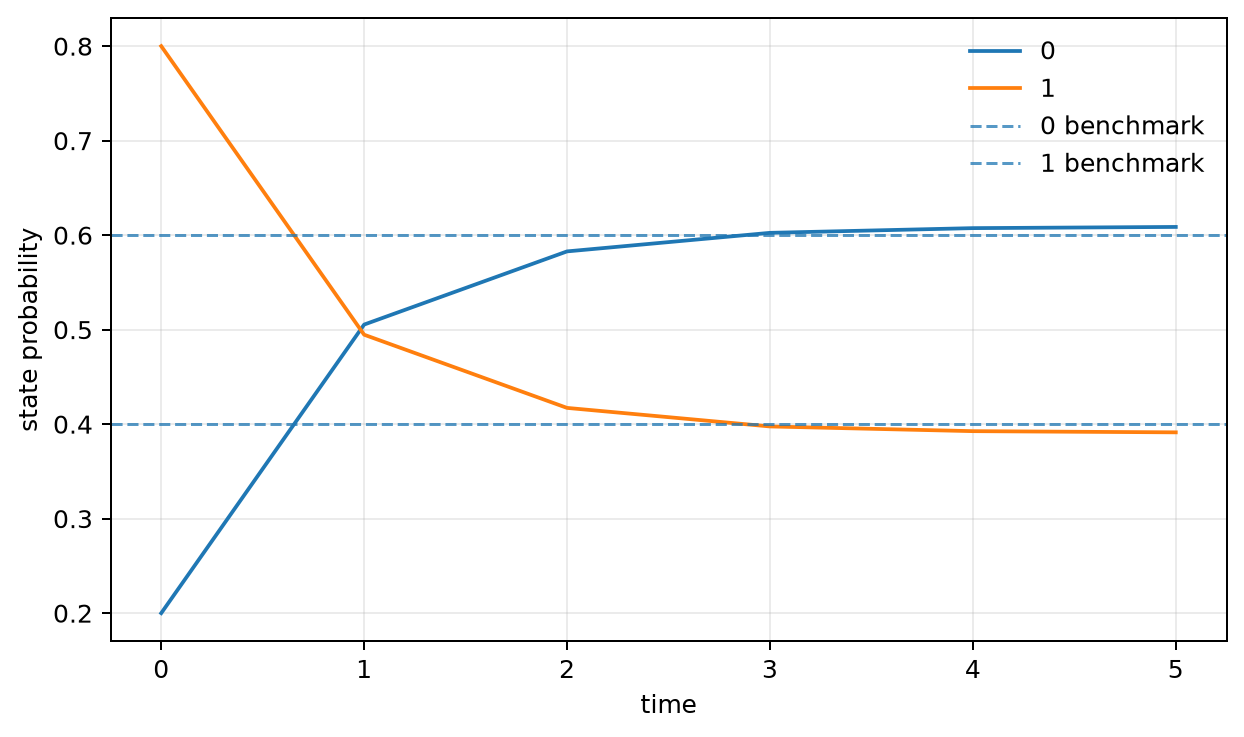
\includegraphics[width=0.34\linewidth]{twostate_flow_mfreinforce.png} \\[3pt]
\textbf{Fixed-scale transport} & \textbf{Adaptive transport} \\[2pt]
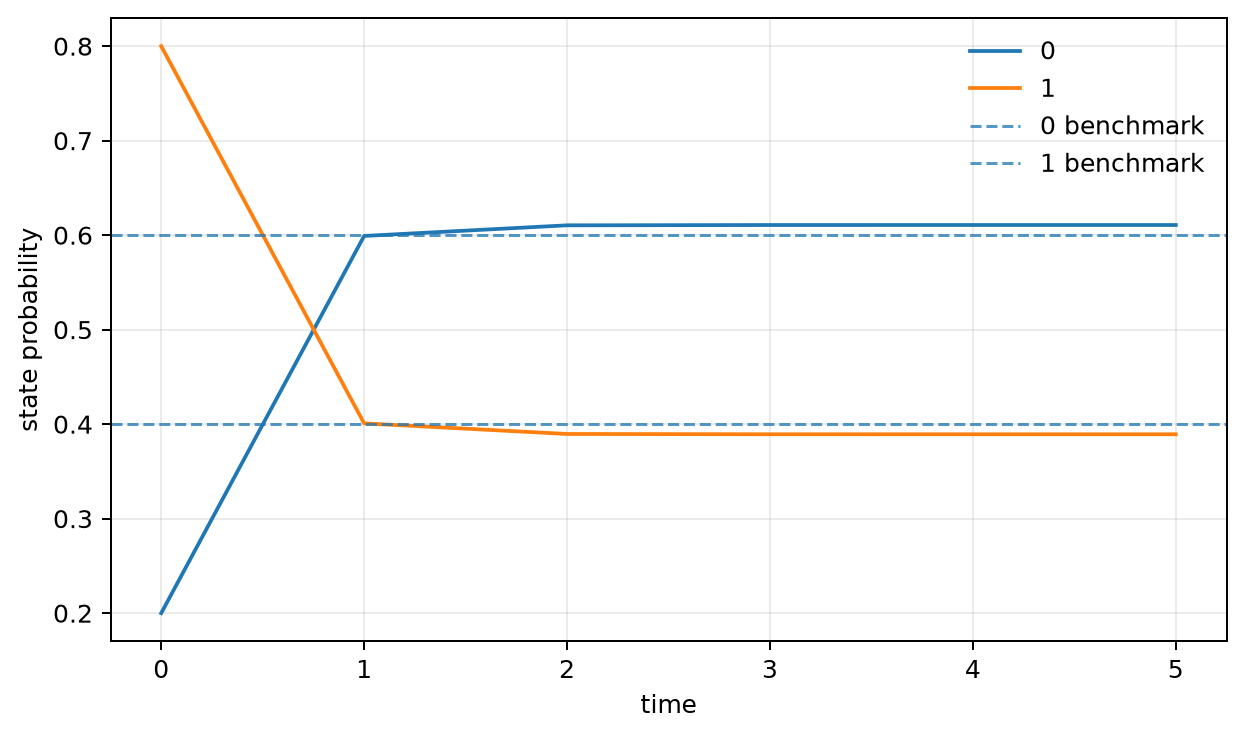
\includegraphics[width=0.34\linewidth]{twostate_flow_transport.png} &
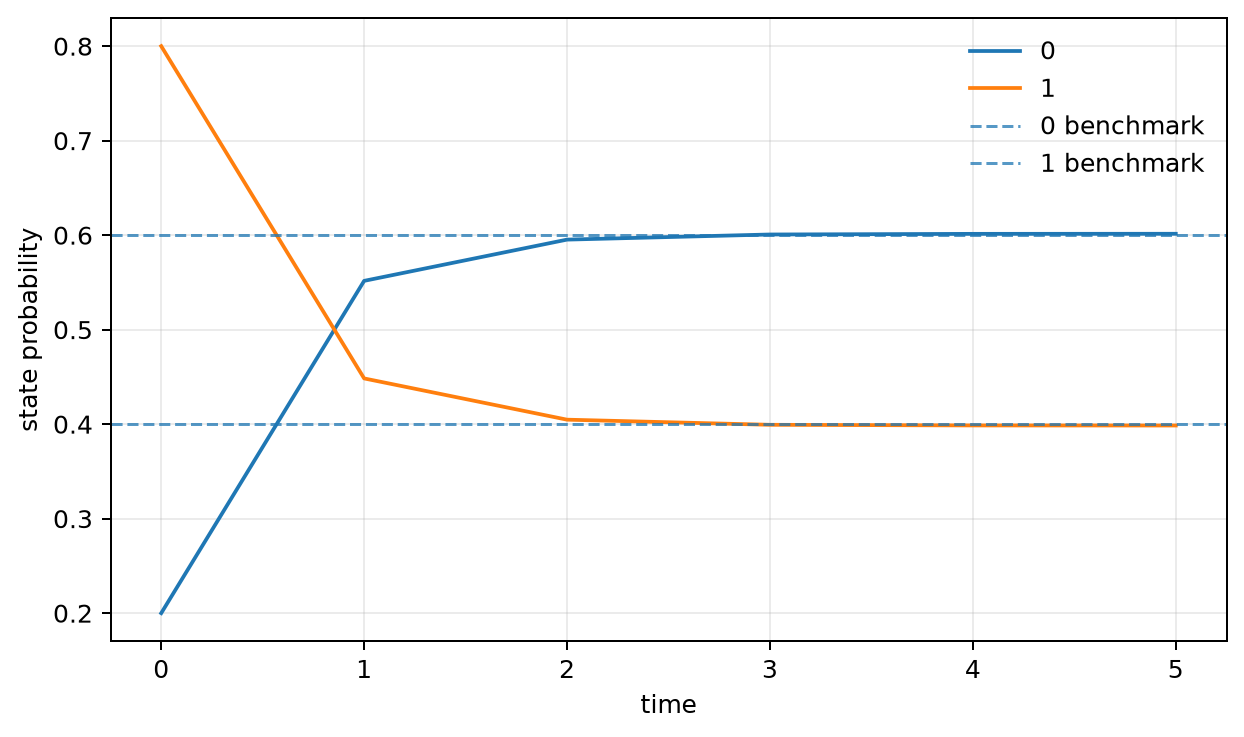
\includegraphics[width=0.34\linewidth]{twostate_flow_adaptive.png}
\end{tabular}
\end{exhibit}

\vspace{-0.05cm}
\scriptsize
The reference policy holds the state-$0$ mass near $0.6$ after the first transition. REINFORCE drives the flow to the wrong corner; the population-aware estimators recover the qualitative target dynamics.
\end{frame}

\begin{frame}{Appendix: Distribution Planning Terminal Law}
\small
\begin{exhibit}{Terminal population law, fixed-scale transport at $\lambda=0.4$}
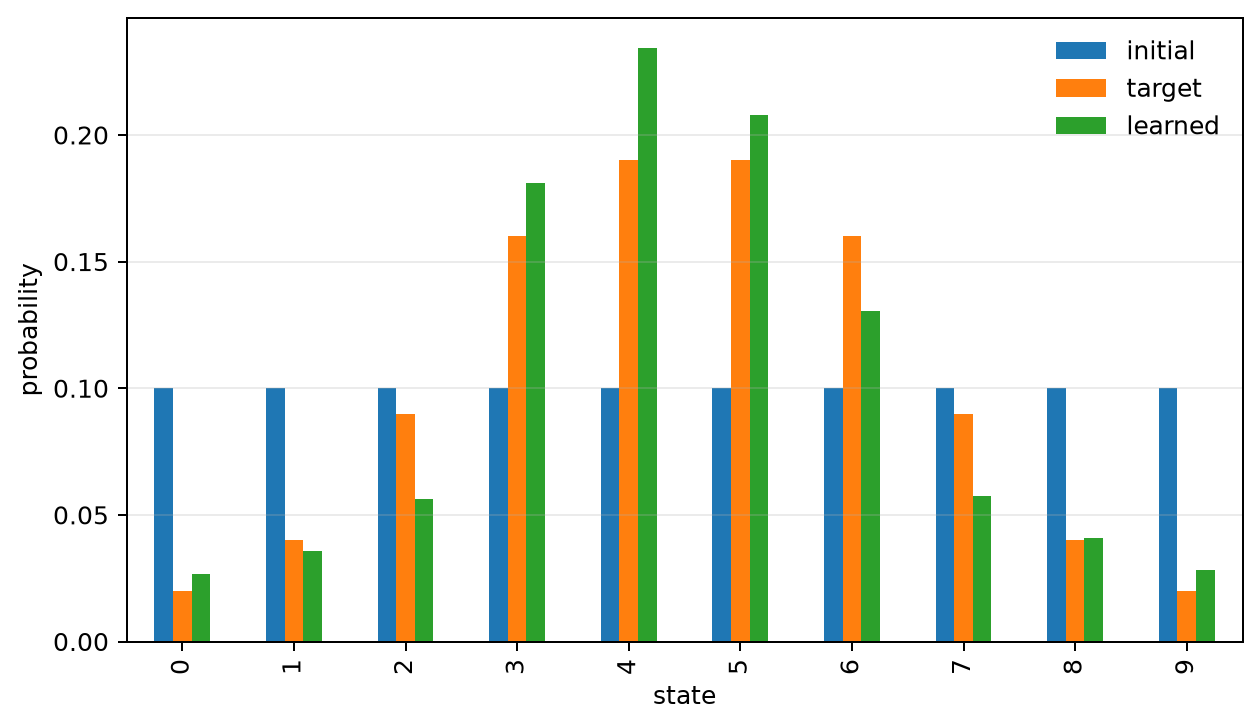
\includegraphics[width=0.58\linewidth]{distribution_terminal_law.png}
\end{exhibit}
\exhibitnote{Against the uniform initial law and the target $\mu_{\rm target}$.}

\vspace{0.1cm}
\small
Transport moves mass in the right qualitative direction. What it cannot do at this budget is estimate the nine-coordinate sensitivity accurately enough to match MF-REINFORCE, which is the second failure mode: the correction is worth having and is not resolvable at $1.2$ auxiliary trajectories per coordinate.
\end{frame}

\begin{frame}{Appendix: Particle-Flow Robustness}
\small
\begin{exhibit}{Exact population recursion replaced by an empirical particle law}
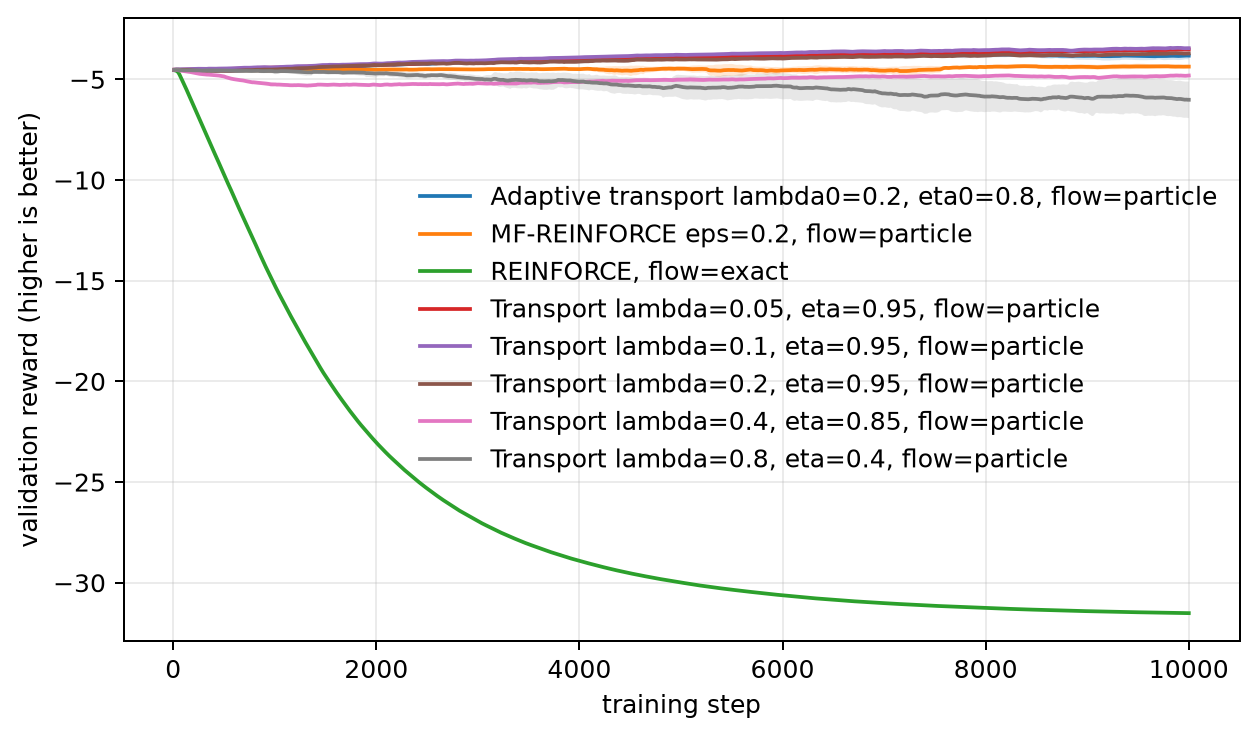
\includegraphics[width=0.44\linewidth]{twostate_validation_T5_particle.png}
\hspace{0.2cm}
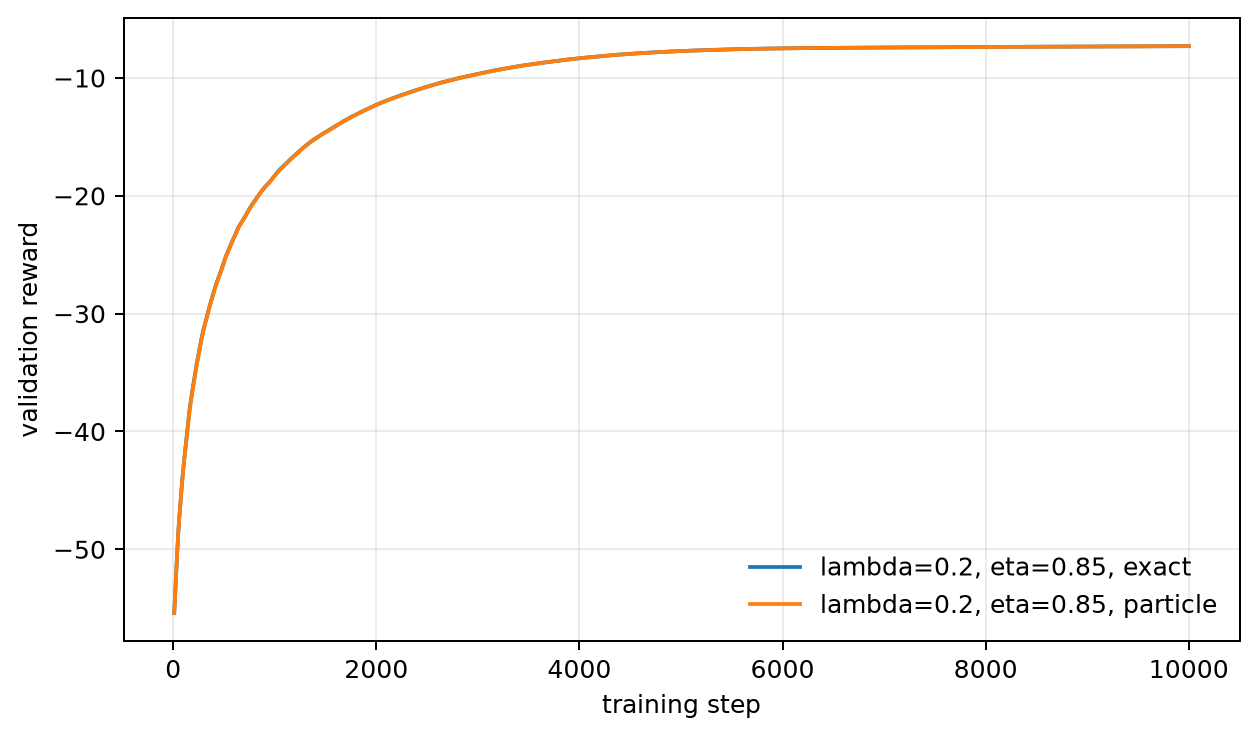
\includegraphics[width=0.44\linewidth]{lq_flow_comparison.png}
\end{exhibit}
\exhibitnote{Left: two-state at $T=5$ with a particle flow. Right: linear--quadratic, exact against particle moment flow.}

\vspace{0.1cm}
\small
The particle approximation is costly on the simplex and nearly free when the population argument is a scalar mean. On two-state at $T=5$ the transport policy error moves from $0.0347$ to $0.0962$, and on the linear--quadratic benchmark the moment flow is essentially unchanged.

\vspace{0.1cm}
In neither case is the population recursion differentiated, which is what keeps the estimator model-free.
\end{frame}

\begin{frame}{Appendix: The Actor--Critic Extension}
\small
In the estimator, the perturbation score is multiplied by the full perturbed return and carries the factor $\lambda^{-1}$ that the MSE decomposition identifies as the dominant variance term at small scales. A deterministic baseline removes only a constant; an advantage from a learned critic would remove the part of the return uninformative about the current step.

\vspace{0.15cm}
The critic is well defined here. The perturbed problem is an ordinary Markov decision process on the augmented space in which the randomized population coordinate is part of the state, so $V^\theta(t,x,m)$ exists and the augmented trajectory law makes this explicit.

\vspace{0.2cm}
Two questions have to be answered before this is a gain:
\begin{itemize}
  \item The critic is evaluated at the perturbed population argument, so its approximation error enters through the same $\lambda^{-1}$ prefactor as the score. The bias it introduces must be traded against the variance it removes, inside the same MSE bound.
  \item The sensitivity recursion has to be revisited, since the critic depends on $\theta$ through the population flow exactly as the reward does.
\end{itemize}

\vspace{0.15cm}
\scriptsize
Closest existing work: the actor--critic algorithms for mean-field control of Pham et al., where the critic is a network reading moments of the population law.
\end{frame}

\begin{frame}{Appendix: A Benchmark with a Two-Dimensional Law Statistic}
\small
Both continuous benchmarks are driven by the population mean, so the chart is one-dimensional and the auxiliary recursion estimates a single scalar flow. Nothing in the suite tests what happens when the law statistic gains a coordinate.

\vspace{0.2cm}
The controlled noisy Kuramoto model is the natural next case. Oscillators on the circle are steered towards synchronization; the state is an angle and the law a distribution on $\mathbb S^1$, but the interaction enters only through the first Fourier mode
\[
  z_t^\theta=\big(\E[\cos X_t^\theta],\ \E[\sin X_t^\theta]\big)\in\R^2 .
\]
So the chart is again exact and finite-dimensional, of dimension two rather than one.

\vspace{0.15cm}
This isolates the question the suite leaves open: does the auxiliary recursion degrade with the dimension of the chart, as the distribution-planning result suggests, and at what rate. It separates that from the confound in distribution planning, where the dimension rises and the state space changes at the same time.
\end{frame}

\end{document}
